%%----------------------------------------------------------------------------------------
%	PACKAGES AND THEMES
%----------------------------------------------------------------------------------------
\PassOptionsToPackage{table}{xcolor}
\documentclass[aspectratio=169,xcolor=dvipsnames,svgnames,x11names,fleqn]{beamer}
% \documentclass[aspectratio=169,xcolor=dvipsnames,fleqn]{beamer}

\usetheme{RedVelvet}

\usefonttheme[onlymath]{serif}
\newcommand{\showanswers}{yes}


\usepackage{xspace}
\usepackage{amsmath}
\usepackage{amssymb}
\usepackage{amsfonts}
\usepackage{color}
\usepackage{physics}
% \usepackage{mathbb}
\usepackage{rahul_math}
\usepackage{bigints}

\usepackage{graphicx} % Allows including images
\usepackage{booktabs} % Allows the use of \toprule, \midrule and \bottomrule in tables
\usepackage{tikz,pgfplots}

\usepackage{subfigure}
\usetikzlibrary{arrows}
\usepackage{minted}
\definecolor{LightGray}{gray}{0.9}
\definecolor{cream}{rgb}{0.92, 0.9, 0.55}
\definecolor{lightblue}{rgb}{0.68, 0.85, 0.9}


\usepackage{xcolor-material}
\usetikzlibrary{fit}
\usetikzlibrary{matrix}
\tikzset{%
apple/.pic={
    \fill [MaterialBrown] (-1/8,0)  arc (180:120:1 and 3/2) coordinate [pos=3/5] (@)-- ++(1/6,-1/7)  arc (120:180:5/4 and 3/2) -- cycle;
    \fill [MaterialLightGreen500] (0,-9/10)  .. controls ++(180:1/8) and ++(  0:1/4) .. (-1/3,  -1) .. controls ++(180:1/3) and ++(270:1/2) .. (  -1,   0) .. controls ++( 90:1/3) and ++(180:1/3) .. (-1/2, 3/4) .. controls ++(  0:1/8) and ++(135:1/8) .. (   0, 4/7)
    }
    }

\newcommand{\leftdoublequote}{\textcolor{blue}{\scalebox{3}{``}}}

\newcommand{\rightdoublequote}{\textcolor{blue}{\scalebox{3}{''}}}


\usepackage{textcomp}
\usepackage{fontawesome}
\usepackage{tikz,pgfplots}
\usetikzlibrary{shapes.callouts}
\usetikzlibrary{arrows}
\usetikzlibrary{shapes.geometric, positioning}
\usetikzlibrary{matrix,positioning,decorations.pathreplacing,calc}

\pgfplotsset{compat=1.8} % or newest version

\usetikzlibrary{positioning}


\usepackage{bm}
\usepackage{relsize}



\tikzset{basic/.style={draw,fill=MediumBlue!20,text width=1em,text badly centered}}
\tikzset{input/.style={basic,circle}}
\tikzset{weights/.style={basic,rectangle}}
\tikzset{functions/.style={basic,circle,fill=MediumBlue!10}}



\usepackage{listofitems} % for \readlist to create arrays
\tikzstyle{mynode}=[thick,draw=MediumBlue,fill=MediumBlue!20,circle,minimum size=22]


\usepackage{overpic}

%----------------------------------------------------------------------------------------
%	TITLE PAGE
%----------------------------------------------------------------------------------------

\usepackage{tikz-qtree,tikz-qtree-compat}
\usetikzlibrary{tikzmark}
\usetikzlibrary{calc}

\usetikzlibrary{fit}
\tikzset{%
apple/.pic={
    \fill [MaterialBrown] (-1/8,0)  arc (180:120:1 and 3/2) coordinate [pos=3/5] (@)-- ++(1/6,-1/7)  arc (120:180:5/4 and 3/2) -- cycle;
    \fill [MaterialLightGreen500] (0,-9/10)  .. controls ++(180:1/8) and ++(  0:1/4) .. (-1/3,  -1) .. controls ++(180:1/3) and ++(270:1/2) .. (  -1,   0) .. controls ++( 90:1/3) and ++(180:1/3) .. (-1/2, 3/4) .. controls ++(  0:1/8) and ++(135:1/8) .. (   0, 4/7)
}
}
\usepackage{tikz-qtree,tikz-qtree-compat}
\usetikzlibrary{tikzmark}
\usetikzlibrary{calc}

\usetikzlibrary{positioning}

% Define styles
\tikzset{
    box/.style={
        rectangle,
        draw=black,
        fill=blue!20,
        text width=2.2cm,
        text centered,
        minimum height=0.8cm,
        font=\small
    },
    arrow/.style={
        ->,
        >=Stealth,
        line width=1.5pt,
        draw=black
    }
}


\usepackage{bm}
\usepackage{relsize}



\tikzset{basic/.style={draw,fill=MediumBlue!20,text width=1em,text badly centered}}
\tikzset{input/.style={basic,circle}}
\tikzset{weights/.style={basic,rectangle}}
\tikzset{functions/.style={basic,circle,fill=MediumBlue!10}}



\usepackage{listofitems} % for \readlist to create arrays
\tikzstyle{mynode}=[thick,draw=MediumBlue,fill=MediumBlue!20,circle,minimum size=22]


\newmdenv[
backgroundcolor=androidYellowLight,
linecolor=androidYellow,
linewidth=0.5pt,
roundcorner=10pt,
skipabove=\baselineskip,
skipbelow=\baselineskip
]{MintedFrame}

% Set minted options
\setminted{
fontsize=\footnotesize,
breaklines=true,
autogobble,
linenos,
frame=none
}


\title[CPE 487/587: Deep Learning]{CPE 486/586: Deep Learning for Engineering Applications} % The short title appears at the bottom of every slide, the full title is only on the title page
\subtitle{05 Deep Learning for Sequence Data}

\author[Rahul Bhadani] {{\Large \textbf{Rahul Bhadani}}}

\institute[UAH] % Your institution as it will appear on the bottom of every slide, maybe shorthand to save space
{
    Electrical \& Computer Engineering,  The University of Alabama in Huntsville
}
\date

% \titlegraphic{
%    \includegraphics[width=0.4\linewidth]{figures/UAH_primary.png}
% }

\begin{document}

%-------------------------------------------------
\begin{frame}
    \titlepage
\end{frame}

%-------------------------------------------------
\begin{frame}{Outline}
    \backgroundtableofcontents
\end{frame}


\section{Motivation}

\begin{frame}
    \sectionpage
\end{frame}

\begin{frame}{Until Now ...}

\begin{enumerate}

\item Data modality: Non-sequential (tabular with no order for samples or features)

\item Process modality: iterative refinement of solution, but not necessarily sequential (non-generative processes -- hence no notion of sequential)


\end{enumerate}

\end{frame}

\begin{frame}{Sequential Data}


\begin{columns}

\column{0.33\linewidth}

    \begin{center}
        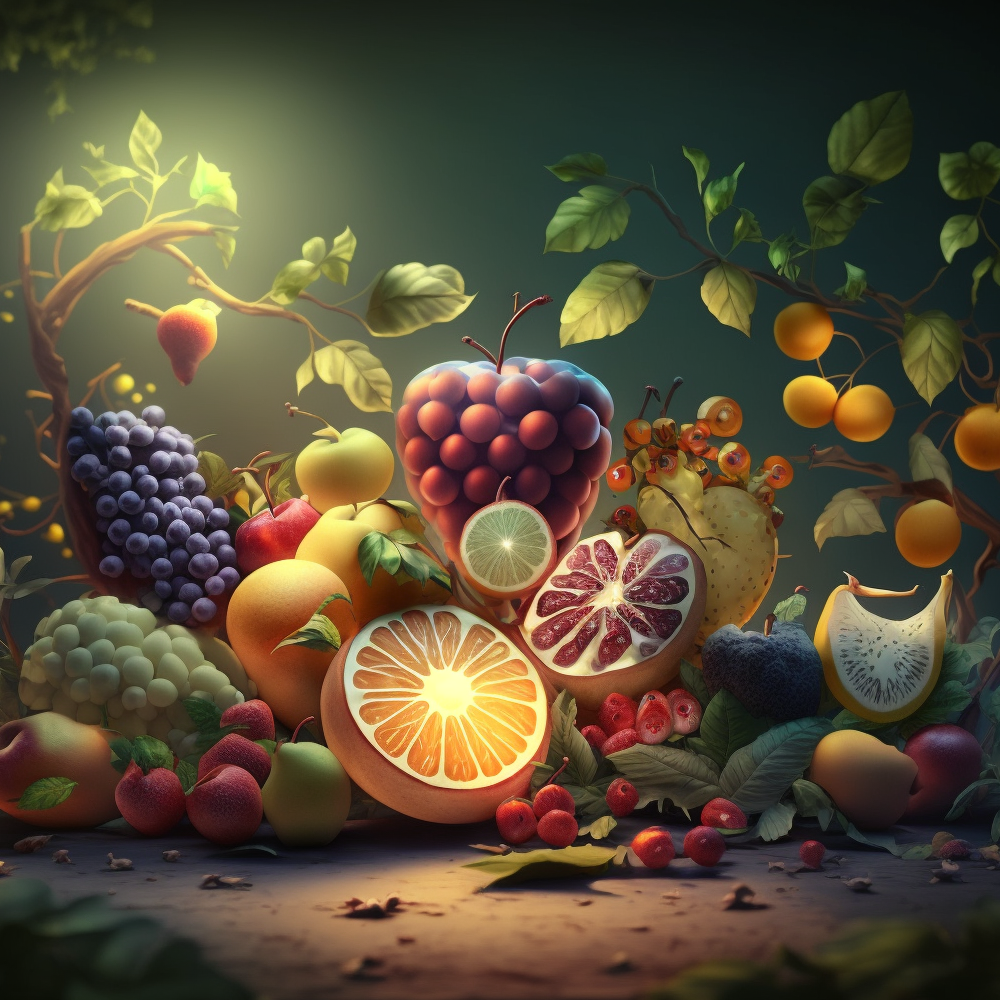
\includegraphics[width=1.0\textwidth]{figures/midjourney_2.png}
        
        Image/Video
   
        
    \end{center}

     
        
\column{0.33\linewidth}

\begin{center}


    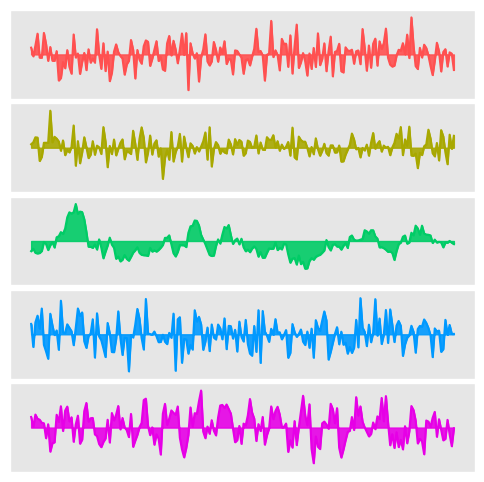
\includegraphics[width=1.0\textwidth]{figures/recreated_signal_plot.png}
    
    Timeseries
    
    \end{center}
    \column{0.33\linewidth}

\begin{center}    
{
    % Set font size to 60pt with 72pt line spacing and make it bold
    \fontsize{15}{15}\selectfont\bfseries

    % Apply a different color to each word using \textcolor{colorname}{text}
    \textcolor{Red}{Efficient}
    \textcolor{Blue}{modelling}
    \textcolor{ForestGreen}{of}
    \textcolor{DarkOrange}{feature}
    \textcolor{Purple}{interactions}
    \textcolor{Teal}{underpins}
}    

\vspace{20pt}
Texts/Natural Language/Computer Code
\end{center}    


        
   
\end{columns} 

\end{frame}


\begin{frame}{Can we use what we learnt so far on Sequential Data?}

Short answer: \textbf{May be!} But not quite!

\vspace{20pt}

{{\textbf{So where is the problem?}}}

\vspace{20pt}


\textbf{\textcolor{DarkOrange}{Underlying Assumptions}}

\vspace{20pt}



\begin{enumerate}
\item Core assumptions have been that data samples are iid (independent and identically distributed)

\item There are also no temporal or spatial dependencies (order of features in the tabular data didn't matter until now).

\item Generally feature length (or number of features are fixed).

\item Non-stationarity assumption: data distribution didn't change.

\end{enumerate}

\end{frame}



\begin{frame}{Learning on Sequential Data}


\begin{enumerate}

\item Images: Convolutional Neural Network (CNN)

\item Texts/Natural language: Recurrent Neural Network (RNN), Long Short-Term Memory (LSTM) Network, Gated Recurrent Unit (GRU) Network, Transformer
\item Videos: CNN + LSTM/GRU/Transformer

\end{enumerate}

\end{frame}


\section{Convolutional Neural Network}

\begin{frame}
    \sectionpage
\end{frame}



\begin{frame}{Convolutional Neural Network}

\begin{center}
    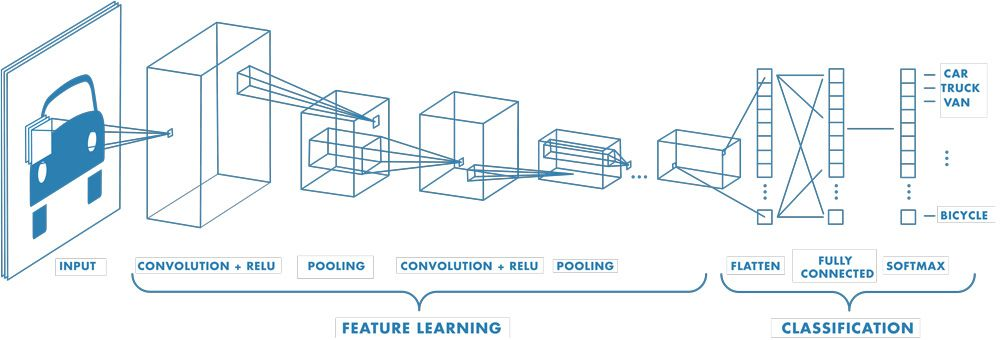
\includegraphics[width=1.0\textwidth]{figures/cnn.jpg}
    
    Source: \url{https://www.mathworks.com/discovery/convolutional-neural-network.html}
\end{center}

\end{frame}

\begin{frame}[fragile]{Motivation for CNN}
\begin{itemize}
        \item \textbf{(Fully-connected Neural Network, FNN Limitation:} Spatial data must be converted to a \textbf{1-D array} (Flattening).
        
        \vspace{0.6cm}
        
        \centering
        \begin{tikzpicture}[
            cell/.style={rectangle, draw=black!60, minimum size=8mm, font=\scriptsize},
            m_matrix/.style={matrix of nodes, nodes={cell, fill=matrixBlue}, column sep=-\pgflinewidth, row sep=-\pgflinewidth},
            % Wider cells for the 1D array to fit the equations
            v_matrix/.style={matrix of nodes, nodes={cell, fill=arrayOrange, minimum width=1.8cm}, column sep=-\pgflinewidth}
        ]
            % 2D Matrix
            \matrix (A) [m_matrix] {
                $a_{11}$ & $a_{12}$ & $a_{13}$ \\
                $a_{21}$ & $a_{22}$ & $a_{23}$ \\
            };
            
            % Flattening Arrow
            \draw[-{Stealth[scale=1.5]}, thick, gray] (A.east) ++(0.1,0) -- node[above, font=\tiny, black] {Flattening} ++(1.1,0);
            
            % 1D Vector with your specific requested labels
            \matrix (B) [v_matrix, right=1.15cm of A, anchor=west] {
                $b_1 = a_{11}$ & $b_2 = a_{12}$ & $b_3 = a_{13}$ & $b_4 = a_{21}$ & $b_5 = a_{22}$ & $b_6 = a_{23}$ \\
            };
            
            % Linking specific elements with the highlight colors
            \node[fill=highlightBlue!30, cell] at (A-1-1) {$a_{11}$};
            \node[fill=highlightBlue!30, cell, minimum width=1.8cm] at (B-1-1) {$b_1 = a_{11}$};
            
            \node[fill=highlightOrange!30, cell] at (A-2-3) {$a_{23}$};
            \node[fill=highlightOrange!30, cell, minimum width=1.8cm] at (B-1-6) {$b_6 = a_{23}$};

        \end{tikzpicture}
        
        \vspace{0.6cm}
        
        \begin{itemize}
            \item[\textcolor{red}{$\times$}] \textbf{Spatial Loss:} We lose the \textcolor{highlightBlue}{pixel-to-pixel relationship} and local geometry.
            \item[\textcolor{red}{$\times$}] \textbf{RGB Complexity:} In addition, working with color images would mean we have at least three channels, R, G, B.
            \item[\textcolor{red}{$\times$}] \textbf{Parameter Explosion:} 
            \begin{itemize}
                \item $200 \times 200 \times 3 = \mathbf{120,000}$ features per image.
                \item Just 100 images = \textcolor{red}{\textbf{12,000,000}} features to process!
            \end{itemize}
        \end{itemize}
    \end{itemize}
\end{frame}

\begin{frame}{Limitations of FNN for Images}

    \begin{columns}
        \column{0.5\linewidth}
        In that sense, FNN suffers from two conditions:
\begin{itemize}
    \item Unable to preserve spatial information
    \item Curse of dimensionality
\end{itemize}

To preserve the pixel-to-pixel spatial relationship, we include two additional operations in the neural network:
\begin{enumerate}
    \item Convolution
    \item Pooling
\end{enumerate}
\column{0.5\linewidth}
\begin{center}
    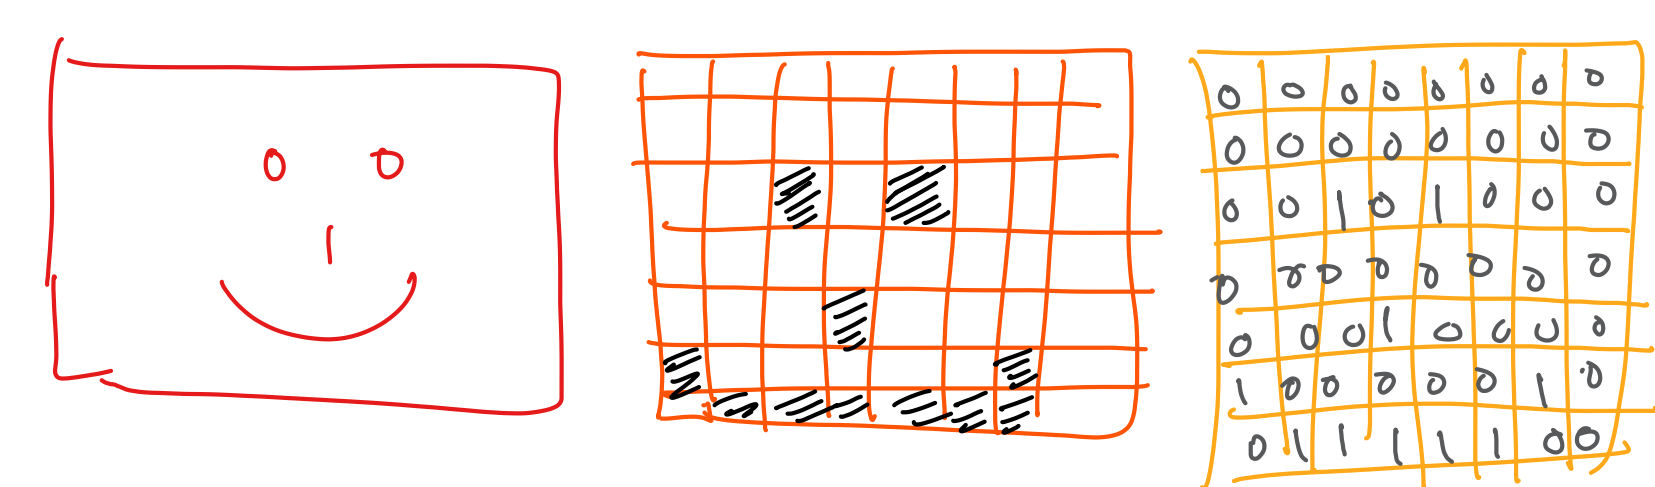
\includegraphics[width=1.0\textwidth]{figures/image_storing.png}
\end{center}
    \end{columns}

\end{frame}

\begin{frame}[fragile]{What is a CNN?}
    \begin{tcolorbox}[colback=mainBlue, colframe=neonBlue, fonttitle=\bfseries, title=Beyond Flattening]
        \color{white}\small
        A \textbf{Convolutional Neural Network (CNN)} is designed for grid-structured data. Unlike FNNs, it treats images as spatial volumes, preserving local relationships.
    \end{tcolorbox}

    \vspace{0.3cm}
    
    \textbf{The Architectural Edge:}
    \begin{itemize}
        \item \textcolor{mainBlue}{\textbf{Local Receptive Fields:}} Neurons only ``see" a small local region, mimicking the human visual cortex.
        \item \textcolor{mainBlue}{\textbf{Spatial Hierarchy:}} Layers learn to recognize edges, then shapes, then objects.
    \end{itemize}

    \vfill
    \centering
    \begin{tikzpicture}[scale=0.6]
        \draw[fill=mainBlue!10, draw=mainBlue] (0,0) grid (3,3);
        \draw[fill=neonBlue!40, draw=neonBlue, line width=1pt] (0,1) rectangle (2,3);
        \node[font=\tiny, text=mainBlue] at (1, 2) {Receptive Field};
        \draw[-Stealth, thick, neonBlue] (2,2) -- (4,2) node[right, font=\tiny, black] {Filter Response};
    \end{tikzpicture}
\end{frame}



\begin{frame}[fragile]{Weight Sharing \& Pooling}
    \begin{columns}[T]
        \begin{column}{0.48\textwidth}
            \begin{tcolorbox}[colback=white, colframe=neonBlue, title=\small Weight Sharing, left=1mm]
                \scriptsize
                Filters share weights across the entire image.
                \begin{itemize}
                    \item \textbf{Efficiency:} Drastically reduces parameters.
                    \item \textbf{Feature Detection:} A vertical edge detector works everywhere!
                \end{itemize}
            \end{tcolorbox}
        \end{column}
        
        \begin{column}{0.48\textwidth}
            \begin{tcolorbox}[colback=white, colframe=neonGreen!70!black, title=\small Pooling, left=1mm]
                \scriptsize
                Subsampling to reduce spatial dimensions.
                \begin{itemize}
                    \item \textbf{Invariance:} Stable against small translations/shifts.
                    \item \textbf{Speed:} Lowers computational load \& memory.
                \end{itemize}
            \end{tcolorbox}
        \end{column}
    \end{columns}

    \vspace{0.4cm}

    \begin{exampleblock}{}
        \centering \small
        \textbf{FNN:} 224x224 image $\approx$ 150k+ weights per neuron. \\
        \textbf{CNN:} 3x3 filter = \textcolor{blue}{\textbf{9 weights}} per feature map.
    \end{exampleblock}
\end{frame}


\begin{frame}{Building blocks: Convolution}

  \begin{columns}
        \column{0.4\linewidth}
    \begin{tblock}{}
        Convolution is an operation to reduce the number of pixels through some operation that, in turn, reduces the number of weights to learn.
    \end{tblock}
    In convolution, the reduction in the number of features happens by sliding a kernel across an image, performing the dot product.


\column{0.6\linewidth}
\textbf{Kernel}: It is an $n \times n$ matrix of some numbers whose dimension is usually smaller than the image size.

\begin{center}
    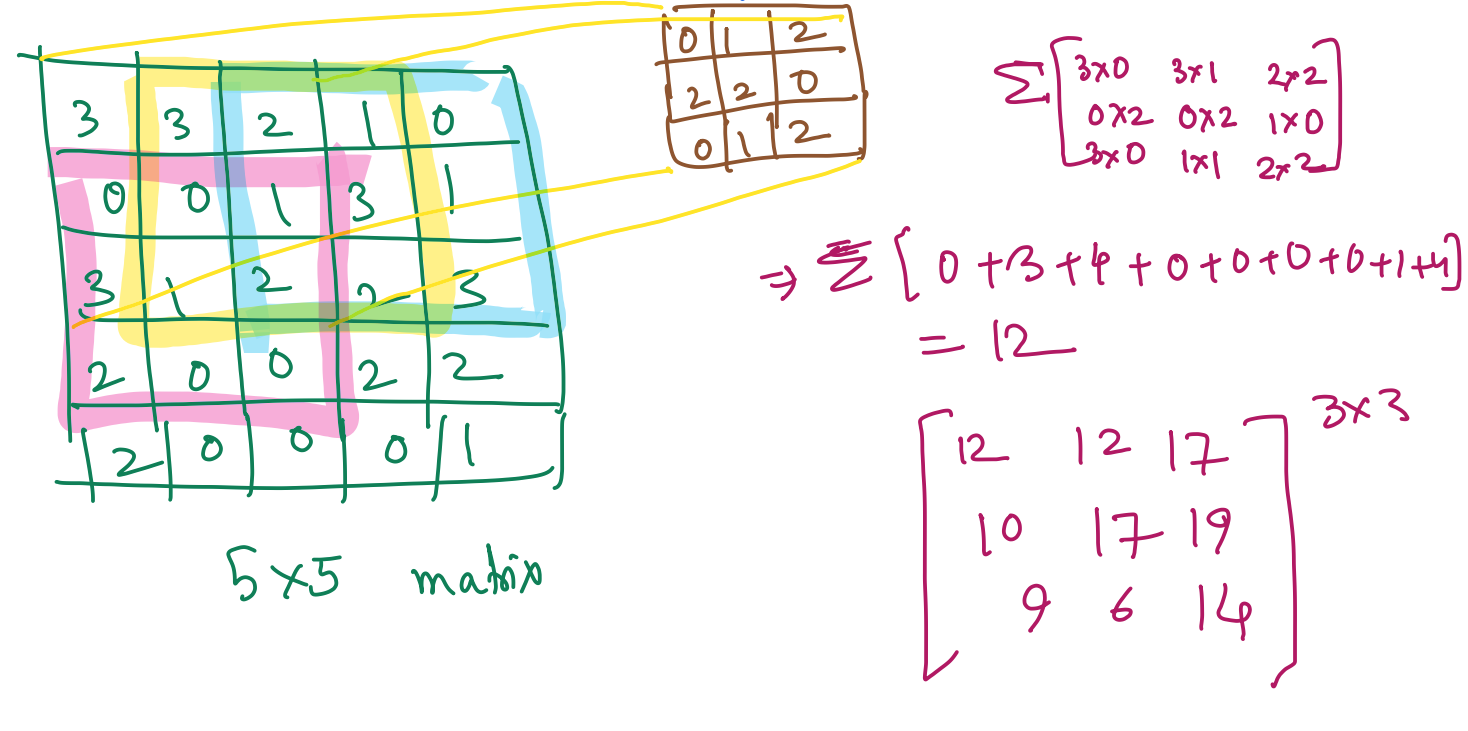
\includegraphics[width=1.0\textwidth]{figures/Kernel.png}
\end{center}

\end{columns}

\end{frame}


\begin{frame}[fragile]{Convolution Using Kernel}
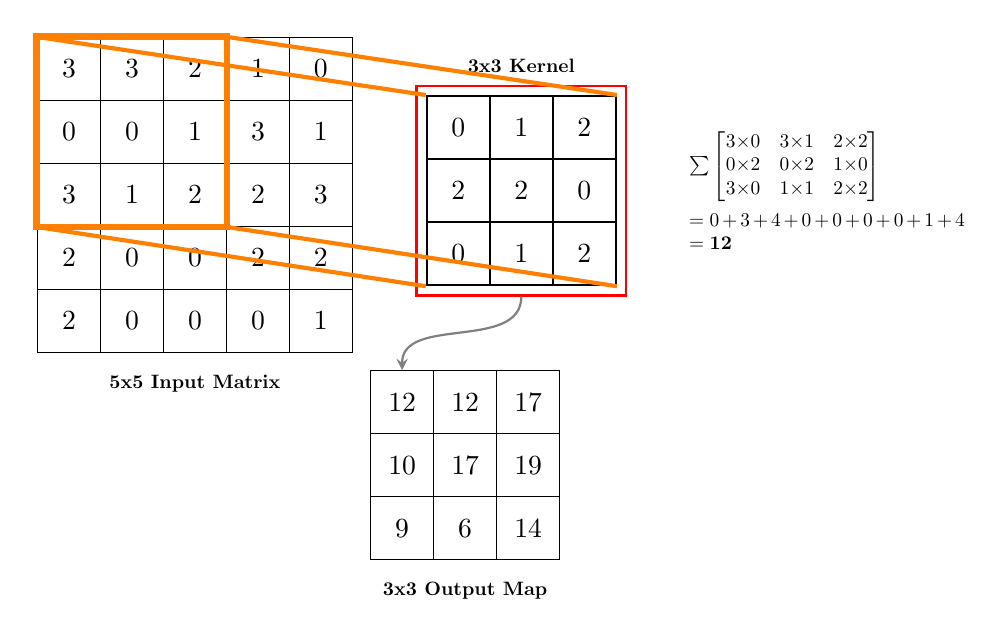
\begin{tikzpicture}[
    scale=0.7, % Change this value to scale everything
    every node/.style={transform shape}, % This is the magic line
    cell/.style={rectangle, draw=black, minimum size=8mm, anchor=center},
    matrix style/.style={
        matrix of nodes, 
        nodes={cell}, 
        column sep=-\pgflinewidth, 
        row sep=-\pgflinewidth, 
        nodes in empty cells
    }
]

% 1. Input Matrix
\matrix (input) [matrix style] {
    3 & 3 & 2 & 1 & 0 \\
    0 & 0 & 1 & 3 & 1 \\
    3 & 1 & 2 & 2 & 3 \\
    2 & 0 & 0 & 2 & 2 \\
    2 & 0 & 0 & 0 & 1 \\
};
\node[below=1mm of input] {\textbf{5x5 Input Matrix}};

% 2. Kernel - Note: I used a relative shift so it scales better
\matrix (kernel) [matrix style, shift={(4,2)}, anchor=north west, draw=red, thick] {
    0 & 1 & 2 \\
    2 & 2 & 0 \\
    0 & 1 & 2 \\
};
\node[above=1mm of kernel] {\textbf{3x3 Kernel}};

% 3. Output Matrix
\matrix (output) [matrix style, shift={(3,-3)}, anchor=north west] {
    12 & 12 & 17 \\
    10 & 17 & 19 \\
    9 & 6 & 14 \\
};
\node[below=1mm of output] {\textbf{3x3 Output Map}};

% 4. Connections
\draw[orange, line width=2.5pt] (input-1-1.north west) rectangle (input-3-3.south east);
\draw[orange, line width=1.5pt] (input-1-1.north west) -- (kernel-1-1.north west);
\draw[orange, line width=1.5pt] (input-1-3.north east) -- (kernel-1-3.north east);
\draw[orange, line width=1.5pt] (input-3-1.south west) -- (kernel-3-1.south west);
\draw[orange, line width=1.5pt] (input-3-3.south east) -- (kernel-3-3.south east);
\draw[->, >=stealth, thick, gray] (kernel.south) to [out=-90, in=90] (output-1-1.north);

% 5. Math Annotation
\node[right=1cm of kernel, text width=5cm] (math) {
    $\sum \begin{bmatrix} 
    3{\times}0 & 3{\times}1 & 2{\times}2 \\
    0{\times}2 & 0{\times}2 & 1{\times}0 \\
    3{\times}0 & 1{\times}1 & 2{\times}2 
    \end{bmatrix}$ \\[2mm]
    $= 0+3+4+0+0+0+0+1+4$ \\
    $= \mathbf{12}$
};

\end{tikzpicture}

\end{frame}


\begin{frame}{Kernels}

    \Large
    \begin{tblock}{}
    A particular kernel usually extracts certain features from an image, or basically, it performs some sort of image processing.
    \end{tblock}

\end{frame}

\begin{frame}{Examples of Kernels}


    \begin{center}
        Edges:  $\begin{bmatrix} 0 & 1 & 0 \\ 1 & -4 & 1 \\ 0 & 1 & 0 \end{bmatrix}$
    \end{center}

    \begin{center}
        Sharpen:      $\begin{bmatrix} 0 & -1 & 0 \\ -1 & 5 & -1 \\ 0 & -1 & 0 \end{bmatrix}$
    \end{center}    
    \begin{center}
        Box Blur:     $\frac{1}{9} \begin{bmatrix} 1 & 1 & 1 \\ 1 & 1 & 1 \\ 1 & 1 & 1 \end{bmatrix}$
    \end{center}


\end{frame}

\begin{frame}{Edge-detection Example}
    \begin{center}
        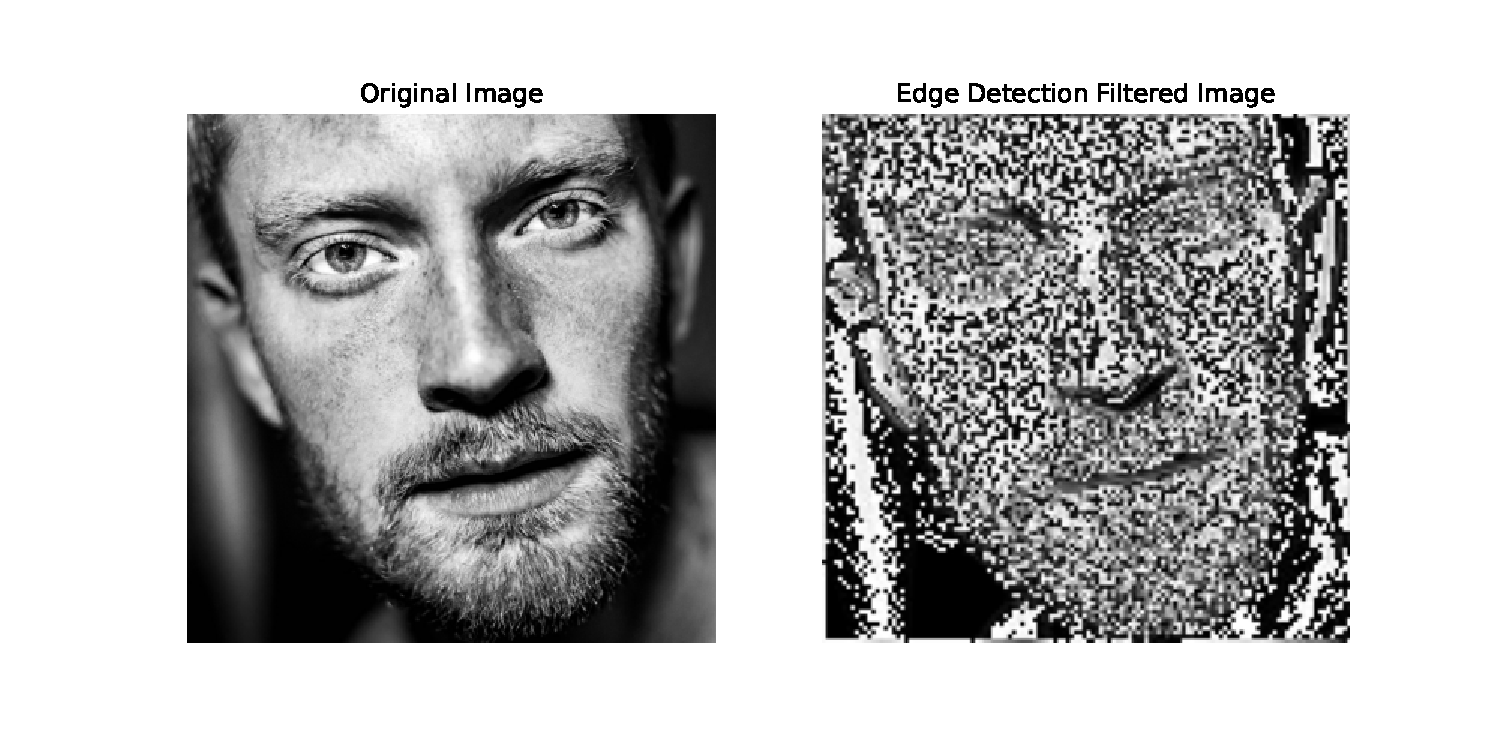
\includegraphics[width=0.7\textwidth]{figures/Edge_detection.pdf}
    \end{center}
\end{frame}


\begin{frame}[fragile]{Filter}
    
    % Header highlight for the introductory text
    \begin{tcolorbox}[colback=bgLight, colframe=accentCyan, arc=2mm, boxrule=0.5pt, left=2mm]
        \small
        The window we use in kernel is called a \textcolor{accentCyan}{\textbf{filter}}. The window of a certain size is slid across the image. We can apply pooling to perform operations such as \textbf{minimum, median, maximum}.
    \end{tcolorbox}

    \vspace{0.4cm}

    \begin{itemize}
        \item \textbf{Images} can be represented as \textcolor{mainNavy}{\textbf{matrices}}, where each element corresponds to a pixel.
        
        \vspace{0.3cm}
        
        \item A \textbf{filter} is just a small matrix that is \textcolor{accentCyan}{\textbf{convolved}} with same-sized sections of the image matrix.
    \end{itemize}

    \vfill

    % Small visual footer to represent the concept
    \centering
    \begin{tikzpicture}[scale=0.5]
        % Background Image Matrix
        \draw[fill=gray!10, draw=gray!40] (0,0) grid (4,3);
        
        % The "Sliding" Filter
        \draw[fill=accentCyan!20, draw=accentCyan, line width=1pt] (1,1) rectangle (2,2);
        
        % Arrow representing sliding
        \draw[-stealth, thick, accentCyan] (2.2, 1.5) -- (3.5, 1.5);
        
        \node[below, font=\tiny, gray] at (2,0) {Image Matrix};
        \node[above, font=\tiny, accentCyan] at (1.5,2) {Filter (Window)};
    \end{tikzpicture}

\end{frame}


\begin{frame}[fragile]{Convolutional Filters}
    \vspace{0.2cm}
    \begin{center}
        \renewcommand{\arraystretch}{1.2}
        % The Operation
        $\begin{bmatrix}
            \cellcolor{windowBlue!80}0 & \cellcolor{windowBlue!80}0 & \cellcolor{windowBlue!80}0 & 0 & 0 & 0 & 0 \\
            \cellcolor{windowBlue!80}0 & \cellcolor{windowBlue!80}1 & \cellcolor{windowBlue!80}2 & 2 & 1 & 1 & 0 \\
            \cellcolor{windowBlue!80}0 & \cellcolor{windowBlue!80}2 & \cellcolor{windowBlue!80}4 & 4 & 2 & 2 & 0 \\
            0 & 1 & 3 & 3 & 1 & 1 & 0 \\
            0 & 1 & 2 & 3 & 1 & 1 & 0 \\
            0 & 0 & 1 & 1 & 0 & 0 & 0
        \end{bmatrix}
        \times 
        \begin{bmatrix}
            \rowcolor{filterGreen} 0 & 1 & 0 \\
            \rowcolor{filterGreen} 1 & -4 & 1 \\
            \rowcolor{filterGreen} 0 & 1 & 0
        \end{bmatrix}
        =
        \begin{bmatrix}
            \cellcolor{windowBlue!80} \mathbf{0} & \dots & \dots \\
            \vdots & \ddots & ~ \\
            \vdots & ~ & \ddots
        \end{bmatrix}$

        \vspace{0.8cm}

        % The Calculation Block
        \begin{minipage}{0.8\textwidth}
            \begin{tcolorbox}[colback=white, colframe=borderBlue!30, arc=1mm, boxrule=0.5pt]
                \centering
                \small
                \textcolor{mathGray}{$(0 \times 0) + (0 \times 1) + (0 \times 0) +$} \\
                \textcolor{mathGray}{$(0 \times 1) + (1 \times -4) + (2 \times 1) +$} \\
                \textcolor{mathGray}{$(0 \times 0) + (2 \times 1) + (4 \times 0) =$} \textbf{\textcolor{borderBlue}{0}}
            \end{tcolorbox}
        \end{minipage}
    \end{center}
\end{frame}

\begin{frame}[fragile]{Convolutional Filters}

\begin{center}
    \renewcommand{\arraystretch}{1.3} % More vertical breathing room
    
    % Input Matrix
    $\begin{bmatrix}
        0 & 0 & 0 & 0 & 0 & 0 \\
       0 & 1 & 2 & 2 & 1 & 0 \\
        0 & 2 & 4 & 4 & 2 & 0 \\
        0 & 1 & 3 & 3 & 1 & 0 \\
        0 & 1 & 2 & 3 & 1 & 0 \\
        0 & 0 & 1 & 1 & 0 & 0
    \end{bmatrix}$
    $\times$ 
    % Filter/Kernel
    $\begin{bmatrix}
       0 & 1 & 0 \\
        1 & -4 & 1 \\
         0 & 1 & 0
    \end{bmatrix}$
    $=$ 
    % Output Matrix
    $\begin{bmatrix}
        \mathbf{\textcolor{resultBlue}{0}} & -1 & -1 & 0\\
        -2 & -5 & -5 & -2\\
        2 & -2 & -1 & 3\\
        -1 & 0 & -5 & 0
    \end{bmatrix}$
    
\end{center}
\end{frame}


\begin{frame}[fragile]{Pooling}
    
    \vspace{0.5cm}
    
    % Use a tcolorbox to frame the definition elegantly
    \begin{tcolorbox}[
        colback=poolLight, 
        colframe=poolGreen, 
        arc=3mm, 
        boxrule=1pt, 
        left=5mm, 
        right=5mm, 
        top=4mm, 
        bottom=4mm
    ]
        \centering
        \color{textDark}
        \large
        \textbf{Pooling} does a mathematical operation on the output of the convolution image. But you can also apply pooling directly to the image.
    \end{tcolorbox}

    \vfill

    % Subtle visual representation of pooling (4 cells into 1)
    \centering
    \begin{tikzpicture}[scale=0.8]
        % Input 2x2
        \draw[fill=gray!10, draw=gray!40] (0,0) grid (2,2);
        \node at (0.5, 1.5) {\tiny 10}; \node at (1.5, 1.5) {\tiny 20};
        \node at (0.5, 0.5) {\tiny 30}; \node at (1.5, 0.5) {\tiny 40};
        
        % Arrow
        \draw[-stealth, thick, poolGreen] (2.5, 1) -- node[above, font=\tiny] {Max Pooling} (4, 1);
        
        % Output 1x1
        \draw[fill=poolGreen!20, draw=poolGreen, line width=1pt] (4.5, 0.5) rectangle (5.5, 1.5);
        \node[poolGreen] at (5, 1) {\small 40};
        
        \node[below=2mm, font=\tiny, gray] at (1,0) {Input Feature Map};
        \node[below=2mm, font=\tiny, poolGreen] at (5,0.5) {Pooled Output};
    \end{tikzpicture}
    
    \vspace{0.3cm}

\end{frame}

\begin{frame}{Building Blocks: Pooling}
    Pooling is a mathematical operation on the output of the convolution image. But you can also apply pooling directly to the image.

\vspace{10pt}

\textbf{Pooling: Downsampling}

\vspace{10pt}

\footnotesize

Combine multiple adjacent nodes into a single node: max-pooling
\begin{multiequation}
    \begin{bmatrix}
        ~ & \cellcolor{blue!30}0 & \cellcolor{blue!30}-1 & -1 & 0\\
        ~ & \cellcolor{blue!30}-2 & \cellcolor{blue!30}-5 & -5 & -2\\
        ~ & 2 & -2 & -1 & 3 \\
        ~ & -1 & 0 & -5 & 0
    \end{bmatrix}
    \to \textbf{max}\to
    \begin{bmatrix}
        ~ & \cellcolor{blue!30}0 & ~\\
        ~ & & ~
    \end{bmatrix}
\end{multiequation}
\begin{multiequation}
    \begin{bmatrix}
        ~ & 0 & 1 & \cellcolor{red!30}-1 & \cellcolor{red!30}-0 & ~\\
        ~ & -2 & -5 & \cellcolor{red!30}-5 & \cellcolor{red!30}-2 & ~\\
        ~ & 2 & -2 & -1 & 3 & ~\\
        ~ & -1 & 0 & -5 & 0 & ~
    \end{bmatrix}
    \to \textbf{max}\to
    \begin{bmatrix}
        ~ & \cellcolor{blue!30}0 & \cellcolor{red!30}0 & ~\\
        ~ & & ~ & ~
    \end{bmatrix}
\end{multiequation}

\begin{itemize}
    \item Reduces the dimensionality of the input to subsequent
    layers and thus, the number of weights to be learned
    \item Further, it protects the network from (slightly) noisy inputs
\end{itemize}
\end{frame}


\begin{frame}[fragile]{Downsampling with Stride}
\begin{itemize}
    \item Only apply the convolution to some subset of the image
    \item e.g., every other column and row = a \textcolor{roseRed}{\textbf{stride of 2}}
\end{itemize}
\vspace{0.3cm}
\centering
\renewcommand{\arraystretch}{1.2}
$ \begin{bmatrix}
    \cellcolor{roseRed!20}0 & \cellcolor{roseRed!20}0 & 0 & 0 & 0 & 0 \\
    \cellcolor{roseRed!20}0 & \cellcolor{roseRed!20}1 & 2 & 2 & 1 & 0 \\
    0 & 2 & 4 & 4 & 2 & 0 \\
    0 & 1 & 3 & 3 & 1 & 0 \\
    0 & 1 & 2 & 3 & 1 & 0 \\
    0 & 0 & 1 & 1 & 0 & 0
    \end{bmatrix} \times \begin{bmatrix} 0 & 1 \\ 1 & -2 \end{bmatrix} =  
    \begin{bmatrix} 
    \cellcolor{roseRed!20}-2 & \textcolor{gray}{\cdot} & \textcolor{gray}{\cdot} \\ 
    \textcolor{gray}{\cdot} & \textcolor{gray}{\cdot} & \textcolor{gray}{\cdot} \\ 
    \textcolor{gray}{\cdot} & \textcolor{gray}{\cdot} & \textcolor{gray}{\cdot} 
    \end{bmatrix} $
\end{frame}    

% --- Slide 2 ---
\begin{frame}[fragile]{Downsampling with Stride}
\centering
\vspace{0.5cm}
\renewcommand{\arraystretch}{1.2}
$ \begin{bmatrix}
    0 & 0 & \cellcolor{pineGreen!20}0 & \cellcolor{pineGreen!20}0 & 0 & 0 \\
    0 & 1 & \cellcolor{pineGreen!20}2 & \cellcolor{pineGreen!20}2 & 1 & 0 \\
    0 & 2 & 4 & 4 & 2 & 0 \\
    0 & 1 & 3 & 3 & 1 & 0 \\
    0 & 1 & 2 & 3 & 1 & 0 \\
    0 & 0 & 1 & 1 & 0 & 0
    \end{bmatrix} \times \begin{bmatrix} 0 & 1 \\ 1 & -2 \end{bmatrix} =   
    \begin{bmatrix} 
    -2 & \cellcolor{pineGreen!20}-2 & \textcolor{gray}{\cdot} \\ 
    \textcolor{gray}{\cdot} & \textcolor{gray}{\cdot} & \textcolor{gray}{\cdot} \\ 
    \textcolor{gray}{\cdot} & \textcolor{gray}{\cdot} & \textcolor{gray}{\cdot} 
    \end{bmatrix} $
\end{frame}    
    
% --- Slide 3 ---
\begin{frame}[fragile]{Downsampling with Stride}
\centering
\vspace{0.5cm}
\renewcommand{\arraystretch}{1.2}
$ \begin{bmatrix}
    0 & 0 & 0 & 0 & \cellcolor{MediumBlue!20}0 & \cellcolor{MediumBlue!20}0 \\
    0 & 1 & 2 & 2 & \cellcolor{MediumBlue!20}1 & \cellcolor{MediumBlue!20}0 \\
    0 & 2 & 4 & 4 & 2 & 0 \\
    0 & 1 & 3 & 3 & 1 & 0 \\
    0 & 1 & 2 & 3 & 1 & 0 \\
    0 & 0 & 1 & 1 & 0 & 0
    \end{bmatrix} \times \begin{bmatrix} 0 & 1 \\ 1 & -2 \end{bmatrix} =   
    \begin{bmatrix} 
    -2 & -2 & \cellcolor{MediumBlue!20} 1 \\ 
    \textcolor{gray}{\cdot} & \textcolor{gray}{\cdot} & \textcolor{gray}{\cdot} \\ 
    \textcolor{gray}{\cdot} & \textcolor{gray}{\cdot} & \textcolor{gray}{\cdot} 
    \end{bmatrix} $
\end{frame}  
        
% --- Slide 4 ---
\begin{frame}[fragile]{Downsampling with Stride}
\centering
\vspace{0.5cm}
\begin{tcolorbox}[colback=white, colframe=gray!20, arc=2mm]
\centering
\renewcommand{\arraystretch}{1.2}
$ \begin{bmatrix}
    0 & 0 & 0 & 0 & 0 & 0 \\
    0 & 1 & 2 & 2 & 1 & 0 \\
    0 & 2 & 4 & 4 & 2 & 0 \\
    0 & 1 & 3 & 3 & 1 & 0 \\
    0 & 1 & 2 & 3 & 1 & 0 \\
    0 & 0 & 1 & 1 & 0 & 0
    \end{bmatrix} \times \begin{bmatrix} 0 & 1 \\ 1 & -2 \end{bmatrix} =   
    \begin{bmatrix} 
    -2 & -2 & 1 \\ 
    0 & 1 & 1 \\ 
    1 & 2 & 0 
    \end{bmatrix} $
\end{tcolorbox}
\end{frame}  

% --- Slide 5 ---
\begin{frame}[fragile]{Operation after Pooling}
    \begin{itemize}
        \item After applying convolution and pooling, we apply a non-linear activation, \textcolor{MediumBlue}{\textbf{ReLU}}.
        \item Then after that, you have more Convolution, more Pooling layers.
        \item Finally, after several sequences of \textbf{Conv + Pool + ReLU}, we \textcolor{roseRed}{\textbf{flatten}} the output and feed it to the fully connected layer (ANN).
    \end{itemize}

    \vfill
    \centering
    \begin{tikzpicture}[node distance=0.4cm, every node/.style={draw, font=\scriptsize\bfseries, inner sep=5pt, rounded corners=1pt}]
        \node[fill=pineGreen!10] (c) {Conv};
        \node[fill=MediumBlue!10, right=of c] (p) {Pool};
        \node[fill=roseRed!10, right=of p] (r) {ReLU};
        \node[draw=none, fill=none, right=of r] (d) {...};
        \node[fill=gray!10, right=of d] (f) {Flatten};
        \node[fill=black, text=white, right=of f] (ann) {ANN};
        
        \foreach \from/\to in {c/p, p/r, r/d, d/f, f/ann}
            \draw[->, >=stealth, thick, gray] (\from) -- (\to);
    \end{tikzpicture}
\end{frame}

\begin{frame}{Image Classification}
Then, we apply a softmax activation if our goal is to do supervised image classification.

\begin{center}
    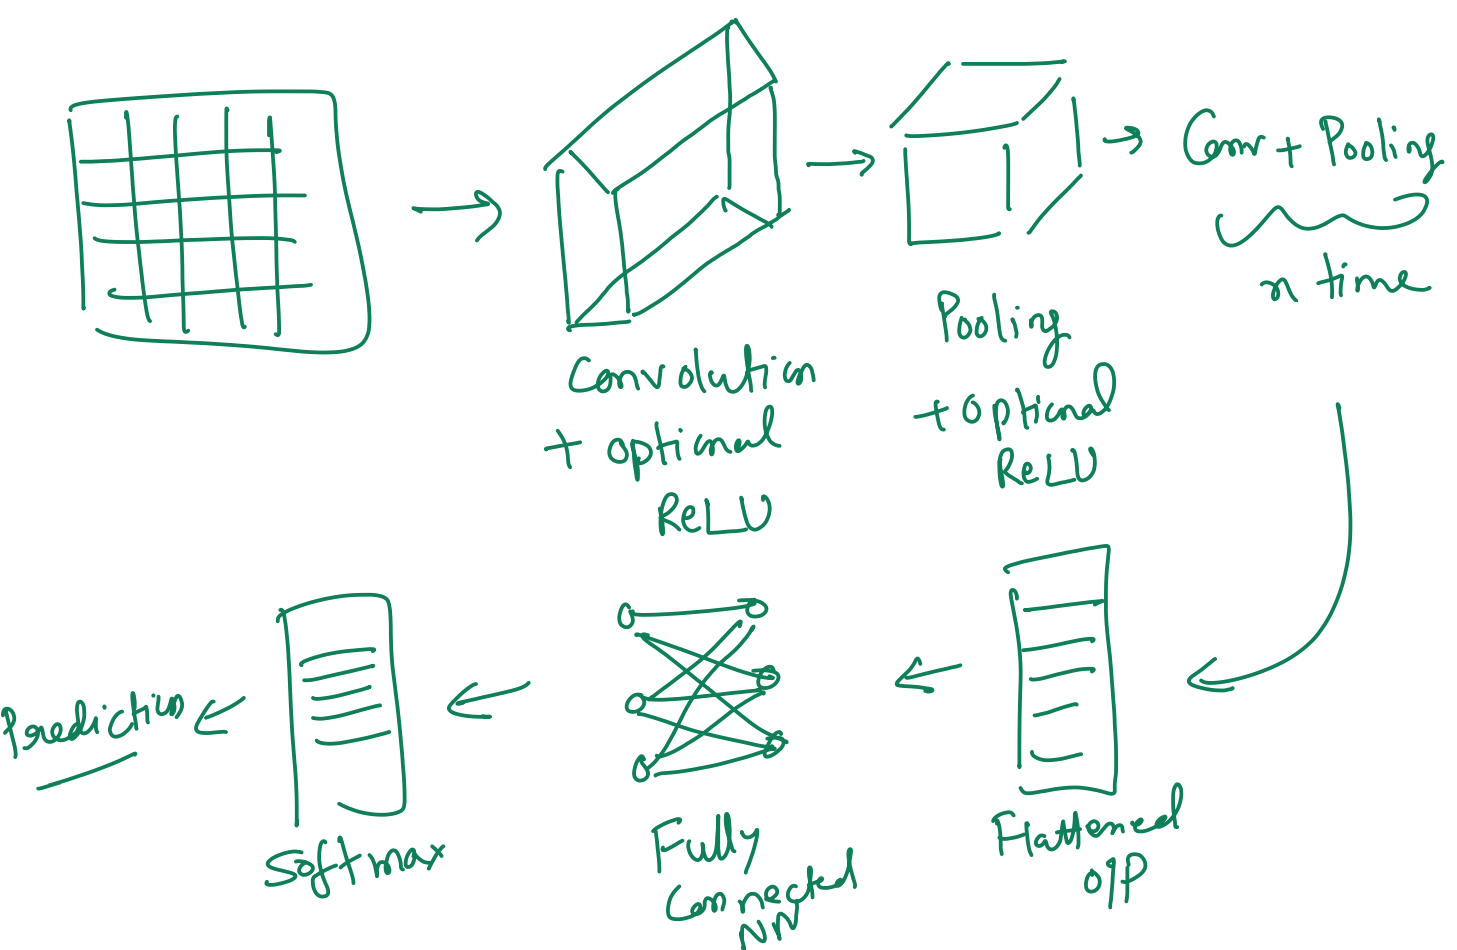
\includegraphics[width=0.52\textwidth]{figures/CNN_Classification_Pipeline.png}
\end{center}

\end{frame}


\begin{frame}{Lenet}
        \begin{center}
            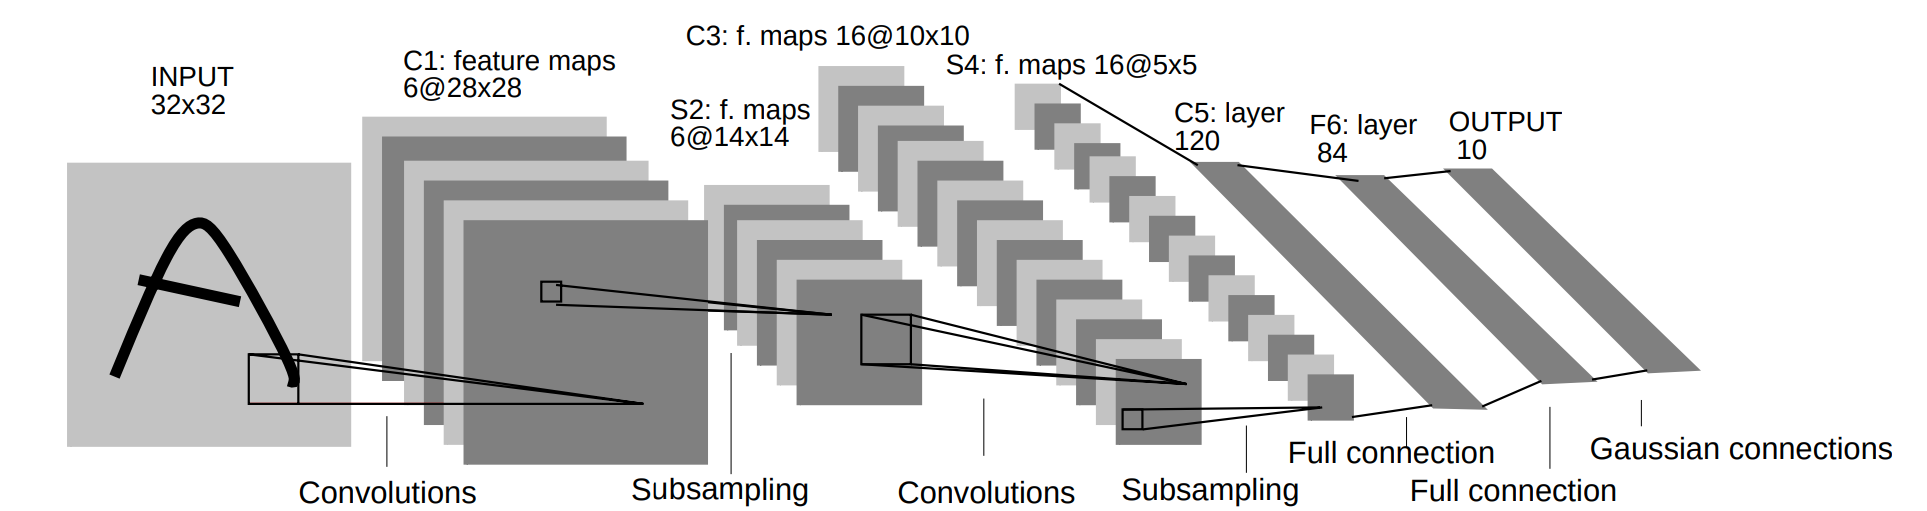
\includegraphics[width=1.0\textwidth]{figures/Lenet.png}
            Source: \url{http://vision.stanford.edu/cs598_spring07/papers/Lecun98.pdf}
        \end{center}
        \begin{itemize}
            \item One of the earliest, most famous deep learning models – achieved remarkable performance at handwritten digit recognition ($< 1$\% test error rate on MNIST dataset)
            \item Used sigmoid (or logistic) activation functions between layers and mean-pooling, both of which are pretty uncommon in modern architectures
        \end{itemize}
        
\end{frame}


\begin{frame}[fragile]{A note on multi-dimensionality and vectorization}
    \begin{itemize}
        \item \textbf{High-Dimensionality:} Images are high-dimensional datasets. This is true even more for \textcolor{indigo}{\textbf{colored images}}.
        \item Let $X \in \mathbb{R}^{H \times W}$ be a matrix (for a grayscale image of height $H$ and width $W$).
        \item \textbf{Flattening:} After flattening, an image is represented as a column vector $X \in \mathbb{R}^{D}$:
        \begin{itemize}
            \item \textbf{Grayscale:} $D = H \times W$
            \item \textbf{Color (3 channels):} $D = H \times W \times 3$
        \end{itemize}
    \end{itemize}
    
    \begin{center}
    \begin{tikzpicture}[scale=0.5]
        \draw[fill=indigo!10] (0,0) rectangle (2,1.5);
        \node at (1, 0.75) {\tiny $H \times W$};
        \draw[->, thick, gray] (2.5, 0.75) -- (4, 0.75);
        \draw[fill=cyanAccent!20] (4.5, -0.5) rectangle (4.8, 2);
        \node[right, font=\tiny] at (4.8, 0.75) {$D$ elements};
    \end{tikzpicture}
    \end{center}
\end{frame}

% --- Slide 2 ---
\begin{frame}[fragile]{Tensor}
    We need a concept of higher-order matrices called a \textcolor{indigo}{\textbf{Tensor}}.

    \begin{itemize}
        \item $X \in \mathbb{R}^{H \times W \times D}$ is an \textbf{order-3 tensor}. Consider it as $D$ channels of matrices. (Note: $D=1$ reduces it to a standard matrix).
    \end{itemize}

    \begin{tcolorbox}[colback=indigo!5, colframe=indigo, title=Tensor Orders]
        \small
        \begin{itemize}
            \item \textbf{Order-0:} A Scalar value.
            \item \textbf{Order-1:} A Vector.
            \item \textbf{Order-2:} A Matrix. \textit{(Corrected from your text)}
            \item \textbf{Order-3:} A Cube (e.g., RGB Image).
        \end{itemize}
    \end{tcolorbox}
    \small We can also have \textbf{4 dimensions} if we consider opacity (e.g., RGBA in PNG).
\end{frame}

% --- Slide 3 ---
\begin{frame}[fragile]{Tensor to Vector}
    Given a tensor, we can arrange all numbers into a long vector following a \textbf{prespecified order}.

    \vspace{0.3cm}
    \textbf{Example (Matrix Vectorization - Column First Order):}
    \begin{center}
        \renewcommand{\arraystretch}{1.2}
        $A = \begin{bmatrix} \textcolor{indigo}{1} & \textcolor{cyanAccent}{2} \\ \textcolor{indigo}{3} & \textcolor{cyanAccent}{4} \end{bmatrix} \xrightarrow{\text{MATLAB } A(:)} \begin{bmatrix} \textcolor{indigo}{1} \\ \textcolor{indigo}{3} \\ \textcolor{cyanAccent}{2} \\ \textcolor{cyanAccent}{4} \end{bmatrix}$
    \end{center}
    
    \begin{exampleblock}{Recursive Vectorization}
        \small
        To vectorize an \textbf{order-3 tensor}, we vectorize the first channel (matrix), then the second, and so on. This recursive process applies to tensors of any order $> 3$.
    \end{exampleblock}
\end{frame}

% --- Slide 4 ---
\begin{frame}[fragile]{Tensor in CNN}
    In CNNs, the convolution kernel will form an \textcolor{amber!80!black}{\textbf{order-4 tensor}}.

\begin{tcolorbox}[colback=white, colframe=cyanAccent, title=CNN Input Dimensions]
\begin{enumerate}
    \item \textbf{Depth:} Number of channels in a colored image.
    \item \textbf{Filters:} Multiple filters learning specific features.
    \item \textbf{Spatial Dimensions:} $H \times W$ of the image.
\end{enumerate}
\end{tcolorbox}

\textbf{Tensor Orders (Examples):}
\begin{itemize}
    \item \textbf{Order 3:} A \textcolor{indigo}{batch} of grayscale images.
    \item \textbf{Order 4:} A \textcolor{indigo}{batch} of colored images or a single colored movie.
    \item \textbf{Order 5:} A \textcolor{indigo}{batch} of movies.
\end{itemize}
\end{frame}

% --- Slide 5 ---
\begin{frame}[fragile]{Tensors}
    \begin{center}
        \begin{tcolorbox}[colback=white, colframe=gray!20, boxrule=0.5pt]
            \centering
            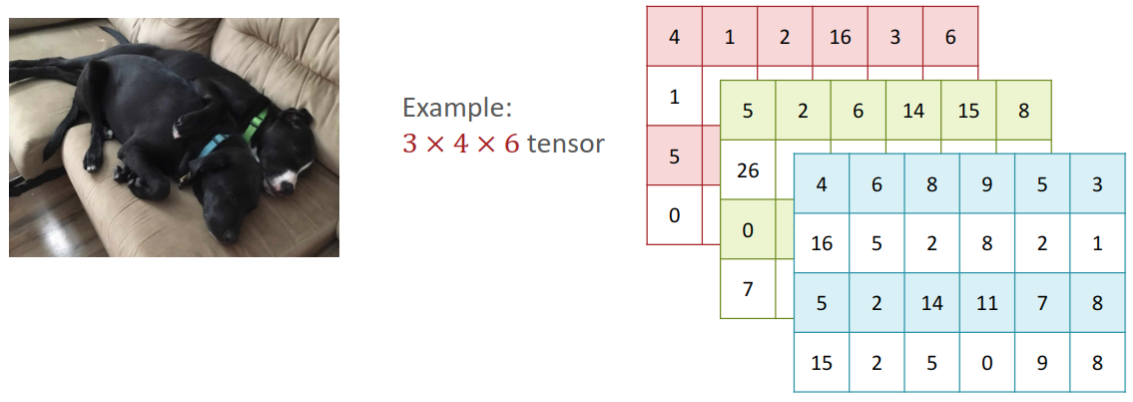
\includegraphics[width=0.75\textwidth]{figures/TensorsRGB.png}
        \end{tcolorbox}
        \vfill
        \tiny \textcolor{gray}{Source: \url{https://www.cs.cmu.edu/~mgormley/courses/10601//slides/lecture17-cnn.pdf}}
    \end{center}
\end{frame}

% --- Slide 6 ---
\begin{frame}[fragile]{Further Reading}
    \begin{center}
        \begin{tcolorbox}[colback=indigo!5, colframe=indigo, arc=0mm, center title]
            \centering
            \small
            \url{https://www.cs.toronto.edu/~hinton/absps/NatureDeepReview.pdf} \\[0.3cm]
            \url{http://vision.stanford.edu/cs598_spring07/papers/Lecun98.pdf}
        \end{tcolorbox}
    \end{center}
\end{frame}


\section{Modern Convolutional Neural Network}

\begin{frame}
    \sectionpage
\end{frame}


\begin{frame}[fragile]{Modern Days of CNN Had Arduous Path}
    
    \begin{tcolorbox}[colback=historyGray!5, colframe=historyGray, arc=0mm, leftrule=3pt, rightrule=0pt, toprule=0pt, bottomrule=0pt]
        \small
        \begin{enumerate}
            \item CNN didn't find its popularity easily.
            \item There was a \textbf{lack of good datasets}.
            \item \textcolor{siftOrange!80!black}{\textbf{Kernel and ensemble methods}} were still better until 2012. 
            \item Computer vision pipelines used methods such as \textit{SIFT, SURF, bag of visual words}.
            \item Researchers were using \textbf{hand-crafted features}.
        \end{enumerate}
    \end{tcolorbox}

    \vspace{0.4cm}

    \begin{tikzpicture}[remember picture, overlay]
        \node[xshift=-2cm, yshift=-1.5cm] at (current page.center) {
            \begin{tikzpicture}
                \draw[thick, gray!30, ->] (0,0) -- (8,0);
                \node[below, font=\tiny, gray] at (0,0) {Before 2012};
                \node[below, font=\tiny, alexBlue] at (7.5,0) {2012+};
                \filldraw[alexBlue] (7.5,0) circle (2pt);
            \end{tikzpicture}
        };
    \end{tikzpicture}

    \vspace{0.3cm}

    \begin{tcolorbox}[colback=alexBlue!10, colframe=alexBlue, arc=2mm, title=\small The Paradigm Shift]
        \small
        However, \textbf{LeCun, Hinton, Ng}, and others thought features can be learnt too. \textcolor{alexBlue}{\textbf{AlexNet}} (after Alex Krizhevsky) proved that.
    \end{tcolorbox}

\end{frame}

\begin{frame}[fragile]{Finally Some Interesting and Useful Datasets}
    
    \begin{itemize}
        \item \textcolor{largeData}{\textbf{Large-Scale Benchmarks}}
        \begin{enumerate}
            \item \textbf{ImageNet (2009):} {\scriptsize \url{https://huggingface.co/datasets/ILSVRC/imagenet-1k}}
            \item \textbf{CIFAR-10 \& CIFAR-100:} {\scriptsize \url{https://www.cs.toronto.edu/~kriz/cifar.html}}
            \item \textbf{LAION Dataset:} {\scriptsize \url{https://laion.ai/projects/}} 
        \end{enumerate}
    \end{itemize}

    \begin{tcolorbox}[colback=mnistPurple!5, colframe=mnistPurple!80, arc=2mm]
        \small
        In addition, Yan LeCun used \textbf{MNIST}: \\ 
        {\scriptsize \url{https://github.com/rahulbhadani/CPE490_590_Sp2025/tree/master/Data/MNIST}}
        
        \vspace{5pt}
        We also have \textbf{FashionMNIST}: \\
        {\scriptsize \url{https://github.com/zalandoresearch/fashion-mnist}}
        
        \vspace{5pt}
        \textit{\textcolor{mnistPurple!80!black}{Note: These two are smaller size datasets.}}
    \end{tcolorbox}


\end{frame}


\begin{frame}[fragile]{AlexNet}

\resizebox{!}{0.9\textheight}{
\begin{tikzpicture}[
    % --- Define Styles ---
    base/.style = {rectangle, draw=black, thick, minimum width=3cm, minimum height=0.7cm, align=center, font=\sffamily\small},
    conv/.style = {base, fill=blue!20},   % Light blue for convolution layers
    pool/.style = {base, fill=cyan!40},   % Darker blue/cyan for pooling layers
    fc/.style   = {base, fill=white},     % White for fully connected layers
    arrow/.style = {-{Stealth[scale=1.0]}, thick}
]

% ==========================================
% LEFT ARCHITECTURE: LeNet
% ==========================================
\node[fc] (l_img) {Image ($28 \times 28$)};
\node[conv, above=0.4cm of l_img] (l_c1) {$5 \times 5$ Conv (6), pad 2};
\node[pool, above=0.4cm of l_c1] (l_p1) {$2 \times 2$ AvgPool, stride 2};
\node[conv, above=0.4cm of l_p1] (l_c2) {$5 \times 5$ Conv (16)};
\node[pool, above=0.4cm of l_c2] (l_p2) {$2 \times 2$ AvgPool, stride 2};
\node[fc, above=0.4cm of l_p2] (l_f1) {FC (120)};
\node[fc, above=0.4cm of l_f1] (l_f2) {FC (84)};
\node[fc, above=0.4cm of l_f2] (l_f3) {FC (10)};

% Draw arrows for LeNet
\foreach \source/\dest in {l_img/l_c1, l_c1/l_p1, l_p1/l_c2, l_c2/l_p2, l_p2/l_f1, l_f1/l_f2, l_f2/l_f3}
    \draw[arrow] (\source) -- (\dest);

% ==========================================
% RIGHT ARCHITECTURE: AlexNet
% ==========================================
% Shifted to the right of LeNet
\node[fc, right=2.5cm of l_img] (r_img) {Image ($3 \times 224 \times 224$)};
\node[conv, above=0.4cm of r_img] (r_c1) {$11 \times 11$ Conv (96), stride 4};
\node[pool, above=0.4cm of r_c1] (r_p1) {$3 \times 3$ MaxPool, stride 2};
\node[conv, above=0.4cm of r_p1] (r_c2) {$5 \times 5$ Conv (256), pad 2};
\node[pool, above=0.4cm of r_c2] (r_p2) {$3 \times 3$ MaxPool, stride 2};
\node[conv, above=0.4cm of r_p2] (r_c3) {$3 \times 3$ Conv (384), pad 1};
\node[conv, above=0.4cm of r_c3] (r_c4) {$3 \times 3$ Conv (384), pad 1};
\node[conv, above=0.4cm of r_c4] (r_c5) {$3 \times 3$ Conv (256), pad 1};
\node[pool, above=0.4cm of r_c5] (r_p3) {$3 \times 3$ MaxPool, stride 2};
\node[fc, above=0.4cm of r_p3] (r_f1) {FC (4096)};
\node[fc, above=0.4cm of r_f1] (r_f2) {FC (4096)};
\node[fc, above=0.4cm of r_f2] (r_f3) {FC (1000)};

% Draw arrows for AlexNet
\foreach \source/\dest in {r_img/r_c1, r_c1/r_p1, r_p1/r_c2, r_c2/r_p2, r_p2/r_c3, r_c3/r_c4, r_c4/r_c5, r_c5/r_p3, r_p3/r_f1, r_f1/r_f2, r_f2/r_f3}
    \draw[arrow] (\source) -- (\dest);

% ==========================================
% CAPTION
% ==========================================
\node[below=0.6cm of $(l_img.south)!0.5!(r_img.south)$, font=\sffamily\itshape] 
    {From LeNet (left), AlexNet (right).};

\end{tikzpicture}
}

\end{frame}

\begin{frame}{AlexNet Architecture}

\begin{enumerate}
\item Convolution window shape: $11\times 11$, then $5\times 5$, and then $3\times 3$.
\item Network adds maxpooling of $3\times 3$ with a stride of 2.
\item At the end,  two huge fully connected layers with 4096 outputs.
\item ReLU activation function.
\end{enumerate}

\end{frame}

\begin{frame}[fragile]{Block Thinking}

\footnotesize

% Hierarchy Header
\centering
\begin{tikzpicture}[node distance=0.5cm]
    \node[draw, fill=blockBlue!10, rounded corners] (n) {Neurons};
    \node[right=of n] (a1) {$\to$};
    \node[draw, fill=blockBlue!20, rounded corners, right=of a1] (l) {Layers};
    \node[right=of l] (a2) {$\to$};
    \node[draw, fill=blockBlue!40, text=white, rounded corners, right=of a2, font=\bfseries] (b) {Blocks};
\end{tikzpicture}

\vspace{10pt}

\begin{tcolorbox}[colback=white, colframe=blockBlue, arc=1mm, boxrule=0.5pt]
    Basic building blocks of CNN are sequence of \textbf{(i)} Convolutional layer with padding \textbf{(ii)} a nonlinearity such as a ReLU \textbf{(iii)} a pooling layer such as max-pooling to reduce the resolution.
\end{tcolorbox}

\textcolor{red!80!black}{But pooling layer reduces dimension by $\log_2 d$ for $d$ dimension input, and it can happen fast exponentially.}

\begin{enumerate}
    \item \textbf{Simonyan and Zisserman (2014)} used multiple convolutional layer in between downsampling via max-pooling in the form of block.
    \item \textbf{Two $3 \times 3$ convolution} have same effect as one $5\times 5$ convolution layer: \textcolor{logicGreen!70!black}{\textbf{deep and narrow networks significantly outperform their shallow counterparts.}}
\end{enumerate}

\vspace{5pt}
\begin{tcolorbox}[colback=gray!5, colframe=citeGray, title=\scriptsize Three important papers in that area:, fonttitle=\bfseries]
    \tiny
    \begin{enumerate}
        \item Simonyan, K. \& Zisserman, A. "Very deep convolutional networks for large-scale image recognition." (2014).
        \item Lavin, A. \& Gray, S. "Fast algorithms for convolutional neural networks." (2016).
        \item Liu, Z. et al. "A convnet for the 2020s." (2022).
    \end{enumerate}
\end{tcolorbox}

\end{frame}

\begin{frame}{VGG Block}
\begin{columns}[T]
    % --- Left Column: Text Content ---
    \begin{column}{0.48\textwidth}
        \footnotesize
        \begin{tcolorbox}[colback=vggLightBlue!10, colframe=vggDeepBlue, arc=1mm, boxrule=0.5pt, left=2pt, right=2pt, top=2pt, bottom=2pt]
        VGG Block (\textbf{Simonyan and Zisserman (2014)}), consists of a sequence of convolutions with $3 \times 3$ kernels with padding of 1 (keeping height and width) followed by a $ 2\times 2$ max-pooling layer with stride of 2 (halving height and width after each block). 
        \end{tcolorbox}

        \vspace{5pt}

        \begin{itemize}
            \item VGG Network can be partitioned into two parts: the first consisting mostly of convolutional and pooling layers and the second consisting of fully connected layers that are identical to those in AlexNet. 
            \item But the convolutional layers are grouped in nonlinear transformations that leave the dimensonality unchanged, followed by a resolution-reduction step.
        \end{itemize}
    \end{column}

    % --- Right Column: TikZ Figure ---
    \begin{column}{0.48\textwidth}
        \centering
        \resizebox{\textwidth}{!}{
            \begin{tikzpicture}[
                node distance=0.4cm,
                layer/.style={rectangle, draw=black, thick, minimum width=4.5cm, minimum height=0.6cm, font=\sffamily\small, align=center},
                conv/.style={layer, fill=vggLightBlue},
                pool/.style={layer, fill=vggDeepBlue},
                fc/.style={layer, fill=white},
                container/.style={rectangle, draw=black, thick, inner sep=0.3cm, rounded corners=2pt},
                arrow/.style={-Stealth, thick}
            ]

                % --- VGG BLOCK (LEFT) ---
                \node[conv] (b_c1) {$3 \times 3$ Conv, pad 1};
                \node[draw=none, above=0.3cm of b_c1] (b_dots) {\dots};
                \node[conv, above=0.3cm of b_dots] (b_c2) {$3 \times 3$ Conv, pad 1};
                \node[pool, above=0.3cm of b_c2] (b_p1) {$2 \times 2$ MaxPool, stride 2};
                
                % Container for VGG Block
                \node[container, fit=(b_c1) (b_p1), label={[font=\sffamily]above:VGG block}] (block_box) {};
                
                % Arrows for Block
                \draw[arrow] (b_c1) -- (b_dots);
                \draw[arrow] (b_dots) -- (b_c2);
                \draw[arrow] (b_c2) -- (b_p1);


                % --- VGG FULL ARCHITECTURE (RIGHT) ---
                \coordinate[right=3cm of b_c1] (vgg_start);
                
                % Bottom Block Segment
                \node[conv, right=3cm of b_c1, minimum width=4cm] (v1_1) {};
                \node[draw=none, above=0.1cm of v1_1] (v1_dots) {\tiny \dots};
                \node[conv, above=0.1cm of v1_dots, minimum width=4cm] (v1_2) {};
                \node[pool, above=0.1cm of v1_2, minimum width=4cm] (v1_p) {};
                \node[container, fit=(v1_1) (v1_p)] (v_box1) {};

                % Middle Dots
                \node[draw=none, above=0.6cm of v_box1] (v_mid_dots) {\dots};

                % Top Block Segment
                \node[conv, above=0.6cm of v_mid_dots, minimum width=4cm] (v2_1) {};
                \node[draw=none, above=0.1cm of v2_1] (v2_dots) {\tiny \dots};
                \node[conv, above=0.1cm of v2_dots, minimum width=4cm] (v2_2) {};
                \node[pool, above=0.1cm of v2_2, minimum width=4cm] (v2_p) {};
                \node[container, fit=(v2_1) (v2_p)] (v_box2) {};

                % Fully Connected Layers
                \node[fc, above=0.8cm of v_box2, minimum width=4cm] (fc1) {FC (4096)};
                \node[fc, above=0.4cm of fc1, minimum width=4cm] (fc2) {FC (4096)};
                \node[fc, above=0.4cm of fc2, minimum width=4cm] (fc3) {FC (1000)};
	            \node[above=0.2cm of fc3] (fc4) {VGG};
                
                

                % --- DRAW ARROWS FOR VGG ---
                \draw[arrow] (v_box1) -- (v_mid_dots);
                \draw[arrow] (v_mid_dots) -- (v_box2);
                \draw[arrow] (v_box2) -- (fc1);
                \draw[arrow] (fc1) -- (fc2);
                \draw[arrow] (fc2) -- (fc3);
            \end{tikzpicture}
        }
    \end{column}
\end{columns}
\end{frame}

\begin{frame}{Network in Network (NiN)}

Two main problems with AlexNet and VGGNet:
\begin{enumerate}
\item FCN at the end of the network has tremendous number of parameters.
\item Cannot add FCN earlier in the network otherwise it can destroy spatial information.
\end{enumerate}
NiN:

\begin{enumerate}
\item use  $1\times 1$ convolutions to add local nonlinearities across the channel activations
\item use global average pooling to integrate across all locations in the last representation layer
\end{enumerate}

\end{frame}

\begin{frame}[fragile]{NiN Block}
\begin{columns}[T]
    % --- Left Column: Text Content ---
    \begin{column}{0.55\textwidth}
        \footnotesize
        
        Input/Output of Convolutional layer is 4-d Tensor with no. of samples $\times$ channel $\times$ height $\times$ width. 
        
        \vspace{5pt}
        Input/output of FC layer are 2-D Tensor: no. of samples $\times$ features.

        \vspace{10pt}
        \begin{tcolorbox}[colback=vggLightBlue!10, colframe=vggDeepBlue, arc=1mm, boxrule=0.5pt, left=3pt, right=3pt, top=3pt, bottom=3pt]
        The idea behind NiN is to apply a fully connected layer at each pixel location (for each height and width). The resulting $1 \times 1$ convolution can be thought of as a fully connected layer acting independently on each pixel location.
        \end{tcolorbox}
    \end{column}

    % --- Right Column: TikZ Diagram ---
    \begin{column}{0.4\textwidth}
        \centering
        \resizebox{\textwidth}{!}{
            \begin{tikzpicture}[
                node distance=0.6cm,
                layer/.style={rectangle, draw=black, thick, minimum width=3.8cm, minimum height=0.8cm, font=\sffamily\bfseries, align=center},
                conv/.style={layer, fill=vggLightBlue},
                container/.style={rectangle, draw=black, thick, inner sep=0.4cm, rounded corners=3pt},
                arrow/.style={-Stealth, thick}
            ]

                % --- NiN Block Components ---
                \node[conv] (base_conv) {Conv};
                \node[conv, above=of base_conv] (1x1_a) {$1 \times 1$ Conv};
                \node[conv, above=of 1x1_a] (1x1_b) {$1 \times 1$ Conv};
                
                % --- Container Box ---
                \node[container, fit=(base_conv) (1x1_b), label={[font=\sffamily\large\bfseries]above:NiN block}] (nin_box) {};
                
                % --- Arrows ---
                \draw[arrow] (base_conv) -- (1x1_a);
                \draw[arrow] (1x1_a) -- (1x1_b);
            \end{tikzpicture}
        }
    \end{column}
\end{columns}
\end{frame}

\begin{frame}[fragile]{NiN Model}
    \begin{columns}[T]
        % --- Left Column: Structured Text ---
        \begin{column}{0.58\textwidth}
            \footnotesize
            \begin{itemize}
                \item \textbf{Initial Convolution Sizes:} NiN uses the same initial convolution sizes as AlexNet: 
                \begin{itemize}
                    \item Kernel sizes are $11\times 11$, $5\times 5$ and $3\times 3$ respectively.
                    \item The numbers of output channels match those of AlexNet.
                \end{itemize}
                \item \textbf{Downsampling:} Each NiN block is followed by a max-pooling layer with a stride of 2 and a window shape of $3\times 3$.
                \item \textbf{Architectural Shift:} 
                \begin{itemize}
                    \item NiN avoids fully connected layers altogether.
                    \item Instead, NiN uses a NiN block with a number of output channels equal to the number of label classes.
                    \item Followed by a global average pooling layer, yielding a vector of logits.
                \end{itemize}
            \end{itemize}
            
            \begin{tcolorbox}[colback=vggLightBlue!10, colframe=vggDeepBlue, arc=1mm, boxrule=0.5pt, left=2pt, right=2pt, top=2pt, bottom=2pt]
                \scriptsize
                This design significantly reduces the number of required model parameters, albeit at the expense of a potential increase in training time.
            \end{tcolorbox}
        \end{column}

        % --- Right Column: TikZ Diagram ---
        \begin{column}{0.38\textwidth}
            \centering
            \resizebox{!}{0.85\textheight}{
                \begin{tikzpicture}[
                    node distance=0.6cm,
                    layer/.style={rectangle, draw=black, thick, minimum width=4cm, minimum height=0.45cm, font=\sffamily\scriptsize},
                    conv/.style={layer, fill=vggLightBlue},
                    pool/.style={layer, fill=vggDeepBlue},
                    container/.style={rectangle, draw=black, thick, inner sep=0.15cm},
                    arrow/.style={-Stealth, thick}
                ]
                    % Block 1
                    \node[conv] (b1_1) {$11 \times 11$ Conv (96), stride 4};
                    \node[conv, above=0.1cm of b1_1] (b1_2) {};
                    \node[conv, above=0.1cm of b1_2] (b1_3) {};
                    \node[container, fit=(b1_1) (b1_3)] (c1) {};
                    
                    % Pool 1
                    \node[pool, above=of c1] (p1) {$3 \times 3$ MaxPool, stride 2};
                    
                    % Block 2
                    \node[conv, above=of p1] (b2_1) {$5 \times 5$ Conv (256), pad 2};
                    \node[conv, above=0.1cm of b2_1] (b2_2) {};
                    \node[conv, above=0.1cm of b2_2] (b2_3) {};
                    \node[container, fit=(b2_1) (b2_3)] (c2) {};
                    
                    % Pool 2
                    \node[pool, above=of c2] (p2) {$3 \times 3$ MaxPool, stride 2};
                    
                    % Block 3
                    \node[conv, above=of p2] (b3_1) {$3 \times 3$ Conv (384), pad 1};
                    \node[conv, above=0.1cm of b3_1] (b3_2) {};
                    \node[conv, above=0.1cm of b3_2] (b3_3) {};
                    \node[container, fit=(b3_1) (b3_3)] (c3) {};
                    
                    % Pool 3
                    \node[pool, above=of c3] (p3) {$3 \times 3$ MaxPool, stride 2};
                    
                    % Block 4
                    \node[conv, above=of p3] (b4_1) {$3 \times 3$ Conv (10), pad 1};
                    \node[conv, above=0.1cm of b4_1] (b4_2) {};
                    \node[conv, above=0.1cm of b4_2] (b4_3) {};
                    \node[container, fit=(b4_1) (b4_3)] (c4) {};
                    
                    % Global AvgPool
                    \node[pool, above=of c4] (gap) {Global AvgPool};
                    
                    % Arrows
                    \foreach \x/\y in {c1/p1, p1/c2, c2/p2, p2/c3, c3/p3, p3/c4, c4/gap}
                        \draw[arrow] (\x) -- (\y);
                \end{tikzpicture}
            }
        \end{column}
    \end{columns}
\end{frame}

\begin{frame}{GoogLeNet: Multi-Branch Networks}
\footnotesize
\begin{columns}[T]
    % --- Left Column: Text Content ---
    \begin{column}{0.45\textwidth}
        \scriptsize
        \textit{Szegedy, C. et al. (2015). Going deeper with convolutions. Proceedings of the CVPR (pp. 1–9).}
        
        \vspace{4pt}
        \textbf{Network Structure:}
        \begin{itemize}
            \item \textbf{Stem for data ingestion:} 
            \begin{itemize}
                \item First two or three convolutions.
                \item Operate directly on the image.
            \end{itemize}
            \item \textbf{Body for data processing:} 
            \begin{itemize}
                \item Contains convolution blocks.
                \item It has concatenated multi-branch convolutions.
            \end{itemize}
            \item \textbf{Head for prediction:} 
            \begin{itemize}
                \item Maps features to the required problem.
                \item Handles classification, segmentation, detection, or tracking.
            \end{itemize}
        \end{itemize}

    \end{column}

    % --- Right Column: TikZ Figure ---
    \begin{column}{0.55\textwidth}
        \centering
\begin{figure}
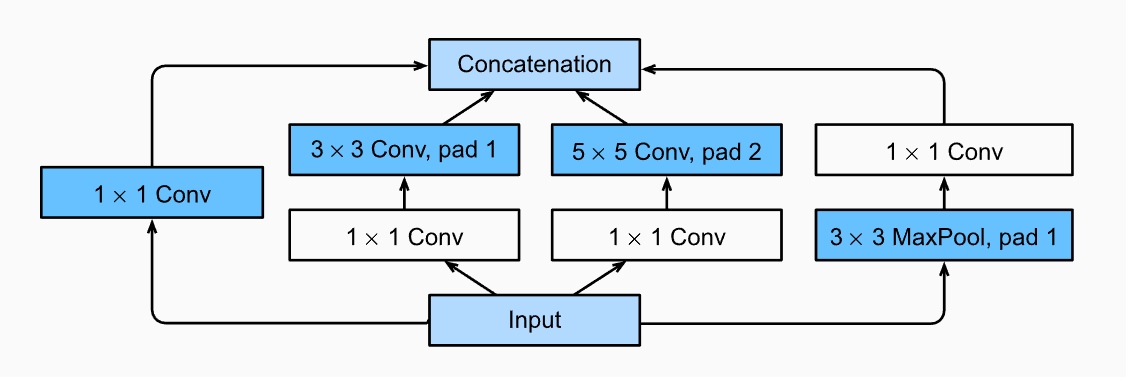
\includegraphics[width=0.99\linewidth]{figures/inception_block.png}
\end{figure}
     \begin{tcolorbox}[colback=vggLightBlue!10, colframe=blockBlue, arc=1mm, boxrule=0.5pt, left=2pt, right=2pt, top=2pt, bottom=2pt]
            \footnotesize
            Convolution block in GoogLeNet is the \textbf{Inception Block}.
        \end{tcolorbox}

    \end{column}
\end{columns}
\end{frame}

\begin{frame}{GoogLeNet Model}

GoogLeNet uses a stack of a total of 9 inception blocks, arranged into three groups with max-pooling in between, and global average pooling in its head to generate its estimates. Max-pooling between inception blocks reduces the dimensionality. At its stem, the first module is similar to AlexNet and LeNet.

\begin{figure}
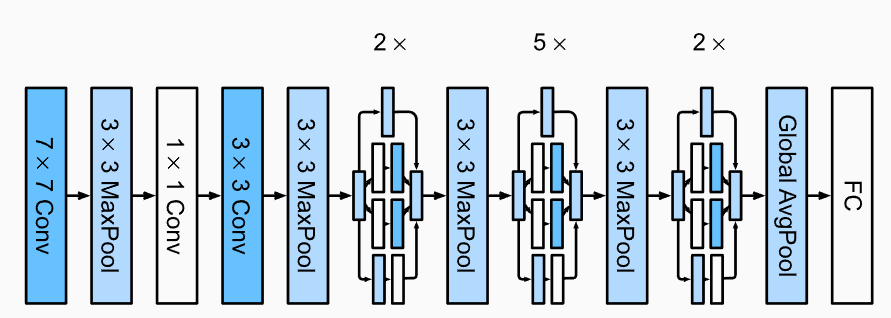
\includegraphics[width=0.79\linewidth]{figures/googlenet.png}
\end{figure}

\end{frame}

\begin{frame}{Applying Batch Normalization in CNN}

\begin{itemize}
    \item \textcolor{blockBlue}{\textbf{Placement:}} With convolutional layers, we can apply batch normalization after the convolution but before the nonlinear activation function.
    
    \item \textcolor{logicGreen!70!black}{\textbf{Per-Channel Logic:}} The key difference from batch normalization in fully connected layers is that we apply the operation on a per-channel basis across all locations.
    
    \item \textcolor{vggDeepBlue}{\textbf{Dimensions:}} 
    \begin{itemize}
        \item Assume minibatches contain $m$ training samples.
        \item For each channel, output height is $p$ and width is $q$.
        \item Normalization is carried out over the \textbf{$m \cdot p \cdot q$} elements per output channel simultaneously.
    \end{itemize}

    \item \textcolor{red!80!black}{\textbf{Spatial Normalization:}} 
    \begin{itemize}
        \item Collect values over all spatial locations to compute mean and variance.
        \item Apply the same mean/variance within a given channel to every spatial location.
    \end{itemize}

    \item \textcolor{citeGray}{\textbf{Parameters:}} Each channel has its own scale and shift parameters, both of which are scalars.
\end{itemize}

\end{frame}

\begin{frame}{Other Advanced CNN Architecture}
    \begin{enumerate}
        \item Xception - Deep Learning with Depthwise Separable Convolutions \url{https://arxiv.org/abs/1610.02357}
        \item DenseNet - Densely Connected Convolutional Neural Networks \url{https://arxiv.org/abs/1608.06993v5}
        \item MobileNetV1 - Efficient Convolutional Neural Networks for Mobile Vision Applications \url{https://arxiv.org/abs/1704.04861v1}
        \item MobileNetV2 - Inverted Residuals and Linear Bottlenecks \url{https://arxiv.org/abs/1801.04381}
        \item ConvNeXt - A ConvNet for the 2020s \url{https://arxiv.org/abs/2201.03545}  
    \end{enumerate}
\end{frame}

\section{Recurrent Neural Network}

\begin{frame}
    \sectionpage
\end{frame}

\begin{frame}{Motivation}
 
  We have seen that Convolutional Neural Networks are effective in capturing spatial relationships in data like images. Further, CNN is good for classification, and regression like tasks are complicated to implement with CNN.

  \bigskip
  However, for data where sequential relationships are important (e.g., text, time series), we need something else.
  

 \begin{center}
    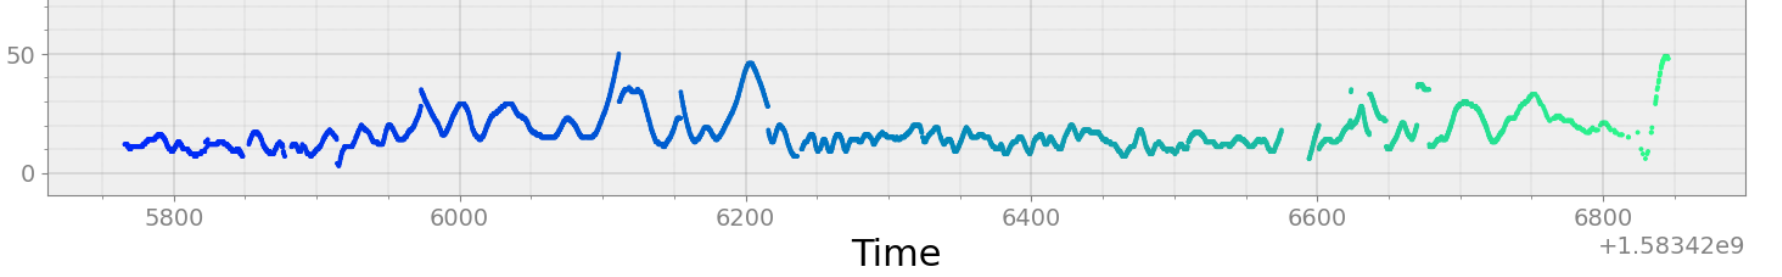
\includegraphics[width=1.0\textwidth]{figures/timeseries.png}
\end{center}
  Timeseries Data.
 \end{frame}
 
 \begin{frame}{Some Example of Sequence Data}

Speech Signal:
 \begin{center}
    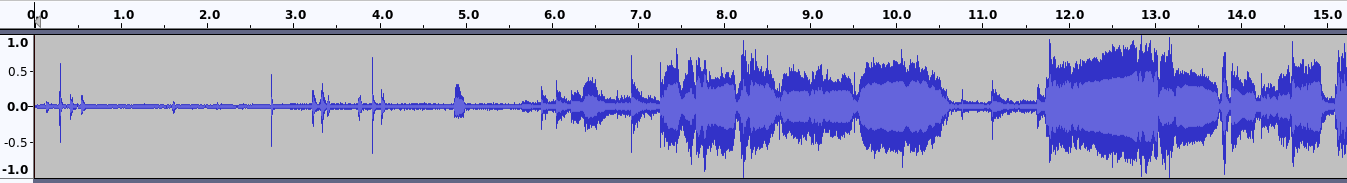
\includegraphics[width=1.0\textwidth]{figures/speech_waveform.png}
\end{center}
Text Sequences:
 \begin{center}
    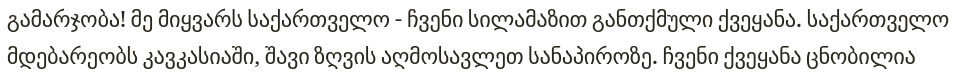
\includegraphics[width=1.0\textwidth]{figures/georgian.png}
\end{center}
 \end{frame}
 
\begin{frame}{Language Model}

    % Clean, structured definition
    \begin{block}{Definition}
        A \textbf{language model} is a machine learning model designed to predict upcoming words in a sequence.
    \end{block}

    \vspace{0.3cm}

    \begin{enumerate}
        \item It assigns a \textbf{probability} to each possible next word, providing a \textit{probability distribution}: $P(w_t \mid w_{1}, \dots, w_{t-1})$.
        \item It can also assign a joint probability to an \textbf{entire sentence}: $P(w_1, \dots, w_n)$.
    \end{enumerate}

    \vspace{0.4cm}
    
    % Using an Example block to differentiate the exercise from the theory
    \begin{exampleblock}{Which has a higher probability of appearing?}
        \centering
        \small
        \textit{"all of a sudden I notice three guys standing on the sidewalk"} \\
        \vspace{0.2cm}
        \textbf{vs.} \\
        \vspace{0.2cm}
        \textit{"on guys all I of notice sidewalk three a sudden standing the"}
    \end{exampleblock}

\end{frame}


\begin{frame}{N-Gram Language Model}
    \vspace{0.2cm}
    
    % Using a block creates a nice visual container for the text
    \begin{block}{Core Objective}
        \begin{itemize}
\item         		Simplest kind of Language Model.
            \item \textbf{Goal:} Generate realistic-looking sentences in human language.
            \item \textbf{Key Idea:} Condition on the last $n-1$ words to sample the $n$-th word.
        \end{itemize}
    \end{block}

    \vfill % Dynamically balances the space between text and image

    \begin{center}
        % Added a thin border/frame around the image for a polished look
        \fbox{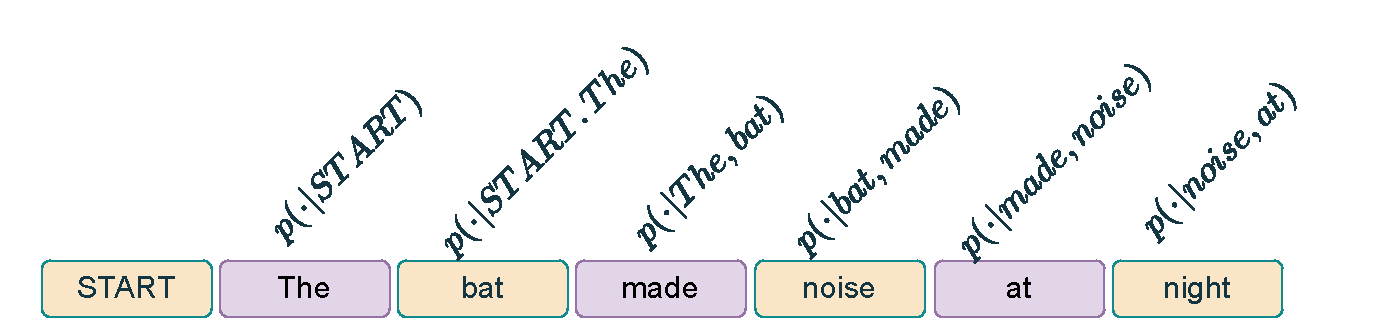
\includegraphics[width=0.85\textwidth, keepaspectratio]{figures/ngram.pdf}}
    \end{center}
    
    \vfill
\end{frame}

\begin{frame}{n-Gram Language Model}
\footnotesize
\textbf{Question}: How can we define a probability distribution over a sequence of length T?
\centering
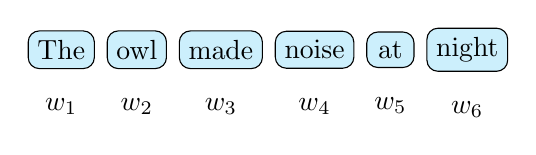
\begin{tikzpicture}[
    node distance=0.25cm and 0.15cm,
    word_box/.style={rectangle, draw, rounded corners, fill=cyan!20, minimum width=0.6cm, minimum height=0.25cm, align=center},
    index_text/.style={below=0.05cm, align=center}
]
    % Words
    \node (w1) [word_box] {The};
    \node (w2) [word_box, right=of w1] {owl};
    \node (w3) [word_box, right=of w2] {made};
    \node (w4) [word_box, right=of w3] {noise};
    \node (w5) [word_box, right=of w4] {at};
    \node (w6) [word_box, right=of w5] {night};

    % Indices
    \node (i1) [index_text, below=of w1] {$w_1$};
    \node (i2) [index_text, below=of w2] {$w_2$};
    \node (i3) [index_text, below=of w3] {$w_3$};
    \node (i4) [index_text, below=of w4] {$w_4$};
    \node (i5) [index_text, below=of w5] {$w_5$};
    \node (i6) [index_text, below=of w6] {$w_6$};

\end{tikzpicture}

\textbf{n - Gram Model (n = 2)}

Using chain rule:
 
 $p(w_1, w_2, ..., w_T) = p(w_1) p(w_2|w_1)p(w_3| w_{1:2})\cdots p(w_n|w_{1:n-1})$
 
$p(w_1, w_2, ..., w_T) = \prod_{t=1}^{T} p(w_t | w_{t-1})$
            
           
$P(w_1, w_2, w_3, w_4, w_5, w_6) =$
\begin{itemize}
    \item $p(w_1)$ \quad \quad (The)
    \item $p(w_2 | w_1)$ \quad (The $\rightarrow$ owl)
    \item $p(w_3 | w_2)$ \quad (owl $\rightarrow$ made)
    \item $p(w_4 | w_3)$ \quad (made $\rightarrow$ noise)
    \item $p(w_5 | w_4)$ \quad (noise $\rightarrow$ at)
    \item $p(w_6 | w_5)$ \quad (at $\rightarrow$ night)
\end{itemize}
\end{frame}


\begin{frame}{n-Gram Language Model}
\footnotesize
\textbf{Question}: How can we define a probability distribution over a sequence of length T?
\centering
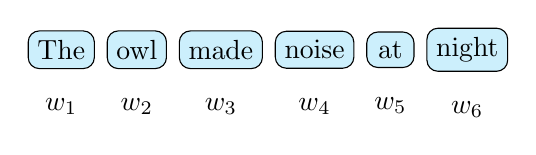
\begin{tikzpicture}[
    node distance=0.25cm and 0.15cm,
    word_box/.style={rectangle, draw, rounded corners, fill=cyan!20, minimum width=0.6cm, minimum height=0.25cm, align=center},
    index_text/.style={below=0.05cm, align=center}
]
    % Words
    \node (w1) [word_box] {The};
    \node (w2) [word_box, right=of w1] {owl};
    \node (w3) [word_box, right=of w2] {made};
    \node (w4) [word_box, right=of w3] {noise};
    \node (w5) [word_box, right=of w4] {at};
    \node (w6) [word_box, right=of w5] {night};

    % Indices
    \node (i1) [index_text, below=of w1] {$w_1$};
    \node (i2) [index_text, below=of w2] {$w_2$};
    \node (i3) [index_text, below=of w3] {$w_3$};
    \node (i4) [index_text, below=of w4] {$w_4$};
    \node (i5) [index_text, below=of w5] {$w_5$};
    \node (i6) [index_text, below=of w6] {$w_6$};

\end{tikzpicture}

\textbf{n - Gram Model (n = 3)}
 
$p(w_1, w_2, ..., w_T) = \prod_{t=1}^{T} p(w_t | w_{t-1}, w_{t-2})$
            
           
$P(w_1, w_2, w_3, w_4, w_5, w_6) =$
\begin{itemize}
    \item $p(w_1)$ \quad \quad (The)
    \item $p(w_2 | w_1)$ \quad (The $\rightarrow$ owl)
    \item $p(w_3 | w_2, w_1)$ \quad (The, owl $\rightarrow$ made)
    \item $p(w_4 | w_3, w_2)$ \quad (owl, made $\rightarrow$ noise)
    \item $p(w_5 | w_4, w_3)$ \quad (made, noise $\rightarrow$ at)
    \item $p(w_6 | w_5, w_4)$ \quad (noise, at $\rightarrow$ night)
\end{itemize}
\end{frame}

\begin{frame}{Learning an n-Gram Model}
\footnotesize



\begin{columns}
\column{0.5\textwidth}
\textbf{Question}: How do we learn the probabilities for the n-Gram Model? \\
\textbf{Answer}: Calculate relative frequencies from training data:

\[
p(w_t | w_{t-n+1}, \dots, w_{t-1}) = \frac{\text{count}(w_{t-n+1}, \dots, w_t)}{\text{count}(w_{t-n+1}, \dots, w_{t-1})}
\]

\textbf{Example: 3-Gram Probabilities} \\
Training corpus with agricultural sentences:
\begin{itemize}
\item ... cows eat grass ... (appears 2 times)
\item ... cows eat hay daily ...(appears 2 times)
\item ... cows eat corn ... (appears 3 times)
\end{itemize}

\column{0.5\textwidth}
\textbf{3-Gram Counts (context: ``cows eat")}:

\begin{tabular}{ll}
\toprule
Next Word & Count \\
\midrule
grass & 2 \\
hay & 2 \\
corn & 3 \\
\bottomrule
\end{tabular}

\vspace{2.5em}

\textbf{Probability Distribution}:

\begin{tabular}{ll}
\toprule
Next Word & Probability \\
\midrule
grass & 0.29 \\
hay & 0.29 \\
corn & 0.43 \\
\bottomrule
\end{tabular}
\end{columns}

\vspace{0.3cm}
\textbf{Calculation}: $ p(\text{corn} | \text{cows eat}) = \frac{3}{7} \approx 0.43 $
\end{frame}


\begin{frame}{Markov Assumption}
\begin{columns}[T]
    % --- Left Column: Text Content ---
    \begin{column}{0.6\textwidth}
        \begin{tcolorbox}[colback=blockBlue!5, colframe=blockBlue, title=Definition, fonttitle=\bfseries, arc=1mm]
            The assumption that the probability of a word depends only on the previous word is called a Markov assumption.
        \end{tcolorbox}

        \vspace{10pt}

        \begin{tcolorbox}[colback=vggDeepBlue!5, colframe=vggDeepBlue, title=Markov Models, fonttitle=\bfseries, arc=1mm]
            Markov models are the class of probabilistic models that assume we can predict the probability of some future unit without looking too far into the past.
        \end{tcolorbox}
    \end{column}

    % --- Right Column: Visual Representation ---
    \begin{column}{0.35\textwidth}
        \centering
        \vspace{1cm}
        \begin{tikzpicture}[
            node distance=1.5cm,
            state/.style={circle, draw=blockBlue, thick, fill=blockBlue!10, minimum size=1cm, font=\footnotesize},
            arrow/.style={-Stealth, thick, shorten >=1pt}
        ]
            % Nodes
            \node[state] (s1) {$w_{t-1}$};
            \node[state, right=of s1] (s2) {$w_{t}$};
            
            % Probabilistic connection
            \draw[arrow] (s1) -- node[above, font=\tiny] {$P(w_t|w_{t-1})$} (s2);
            
            % Self-loops or previous history (grayed out to show exclusion)
            \node[left=0.8cm of s1, color=gray!50] (dots) {\dots};
            \draw[arrow, color=gray!30, dashed] (dots) -- (s1);
            
            \node[below=0.2cm of s1, font=\tiny, color=blockBlue] {Previous};
            \node[below=0.2cm of s2, font=\tiny, color=blockBlue] {Current};
        \end{tikzpicture}
        
        \vspace{5pt}
        \scriptsize \textcolor{citeGray}{Visualizing the first-order dependency.}
    \end{column}
\end{columns}
\end{frame}



\begin{frame}{How to estimate probabilities}

\textbf{Maximum Likelihood Estimation method:}

Count words from a corpus, and normalize the counts so they fall between 0 and 1.

Computing 2-gram probability:

\begin{align*}
p(w_n|w_{n-1}) = \frac{C(w_{n-1}w_n)}{\sum_w C(w_{n-1} w)} = \frac{C(w_{n-1}w_n)}{ C(w_{n-1})} 
\end{align*}
because the sum of all 2-gram counts that start with a given word $w_{n-1}$ is equal to 1-gram count for that word $w_{n-1}$.


\end{frame}

%\begin{frame}{How to estimate probabilities}
%\begin{columns}[T]
%    % --- Left Column: Method and Logic ---
%    \begin{column}{0.5\textwidth}
%        \textcolor{blockBlue}{\textbf{Maximum Likelihood Estimation method:}}
%        
%        \vspace{5pt}
%        \begin{itemize}
%            \item \textbf{Process:} Count words from a corpus, and normalize the counts so they fall between 0 and 1.
%            
%            \vspace{10pt}
%            \item \textbf{Logic:} The sum of all 2-gram counts that start with a given word $w_{n-1}$ is equal to the 1-gram count for that word $w_{n-1}$.
%        \end{itemize}
%    \end{column}
%
%    % --- Right Column: Formula ---
%    \begin{column}{0.48\textwidth}
%        \centering
%        \textbf{Computing 2-gram probability:}
%        
%        \vspace{10pt}
%        \begin{tcolorbox}[colback=vggDeepBlue!5, colframe=vggDeepBlue, arc=1mm, boxrule=0.8pt]
%            \small
%            \begin{align*}
%            p(w_n|w_{n-1}) &= \frac{C(w_{n-1}w_n)}{\sum_w C(w_{n-1} w)} \\
%            &= \frac{C(w_{n-1}w_n)}{ C(w_{n-1})} 
%            \end{align*}
%        \end{tcolorbox}
%        
%        \vspace{5pt}
%        \scriptsize \textcolor{citeGray}{Normalization ensures valid probabilities.}
%    \end{column}
%\end{columns}
%\end{frame}

\begin{frame}[fragile]{Example}


          \begin{minted}[
                linenos,
                frame=lines,
                framesep=2mm,
                bgcolor=pink!10,
                fontsize=\footnotesize,
                breaklines
            ]{html}
            
            <s> I am Sam </s>
            <s> Sam I am </s>
            <s>I do not  like green peas and cheese</s>
\end{minted}

$P(I|<s>) = 2/3 = 0.67, P(<s>|Sam) = 1/2 = 0.5, P(Sam|<s>) = 1/3 = 0.33, P(Sam|am) = 1/2 = 0.5, P(am|I) = 2/3 = 0.67, = 0.5 P(do|I) = 1/3 = 0.33$



\end{frame}

\begin{frame}{Sampling from a Language Model}
\footnotesize

\textbf{Process}:
\begin{enumerate}
\item Start with initial context (n-1 words)
\item Roll weighted die for next word
\item Slide window and repeat
\end{enumerate}

\begin{columns}[T]
\column{0.5\textwidth}
\textbf{Sampling Demonstration}:
\begin{tabular}{lll}
Step & Context & Sampled Word \\
\hline
1 & [START] The & bat \\
2 & The bat & made \\
3 & bat made & noise \\
4 & made noise & at \\
5 & noise at & night \\
6 & at night & [END] \\
\end{tabular}

\column{0.5\textwidth}
\textbf{Generated Sentence}:
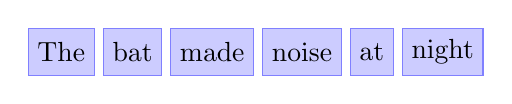
\begin{tikzpicture}[
node distance=0.1cm,
word/.style={rectangle, draw=blue!50, fill=blue!20, minimum height=0.6cm}
]
\node[word] (w1) {The};
\node[word, right=of w1] (w2) {bat};
\node[word, right=of w2] (w3) {made};
\node[word, right=of w3] (w4) {noise};
\node[word, right=of w4] (w5) {at};
\node[word, right=of w5] (w6) {night};
\end{tikzpicture}


Sampling introduces diversity but preserves local coherence through n-gram constraints.

\end{columns}

\end{frame}

\begin{frame}{Recurrent Connections and Recurrent Neural Networks}
  \textbf{Recurrent Connection:}
  Introduction of a cycle in a network.


  \textbf{Recurrent Neural Network (RNN):}
  Any neural network that contains a cycle within its network connection.

  There are many types of RNN. We will see the \textbf{Elman network} (1990, Elman).

  \begin{center}
    \tikzstyle{neuron}=[circle,draw,fill=red!20,minimum size=3.5em,inner sep=0, node distance=2cm]
    \tikzstyle{input}=[rectangle,draw,fill=blue!20,minimum size=3em,inner sep=5pt]

    \begin{tikzpicture}[>=stealth]
      \node[input] (xt) {$x_t$};
      \node[neuron, right=of xt] (ht) {$h_t$};
      \node[neuron, right=of ht] (yt) {$y_t$};

      \draw[->] (xt) -- (ht);
      \draw[->] (ht) -- (yt);
      \draw[->] (ht) to[out=45,in=135,loop] (ht);
    \end{tikzpicture}
  \end{center}

\end{frame}
\begin{frame}{Elman Network}

  The equations for the Elman network are:
  \begin{multiequation}
    h_t &= g(Uh_{t-1} + Wx_t) \\
    y_t &= f(Vh_t)
  \end{multiequation}
  where $g$ is an activation function (e.g., tanh or sigmoid).
  
  At the end, output layer also contains softmax: $y_t = \text{softmax}(Vh_t)$.

  \bigskip
  The goal is to learn the weights $U$, $W$, and $V$.

  \bigskip
  At the end output layer, softmax is often used.
\end{frame}

\begin{frame}{See an Example RNN Network}
  The feedback loop in Recurrent Neural Networks (RNNs) networks makes it possible to establish long-range dependence on sequential data.

  \bigskip
  To understand how these networks process sequential data over time, we can "unroll" the network.
  
  \centering
    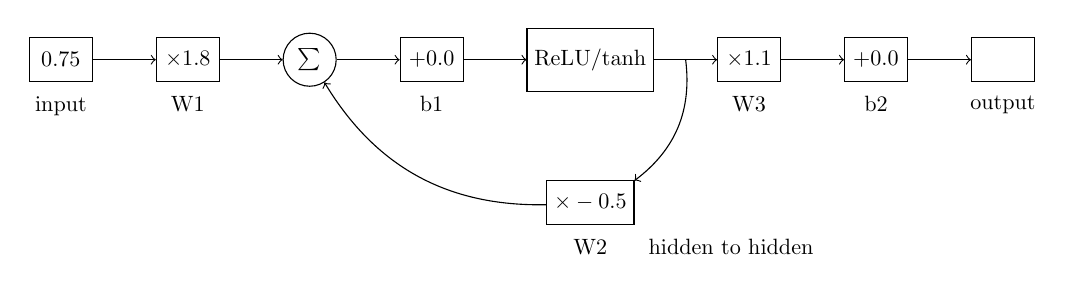
\begin{tikzpicture}[scale=0.8, transform shape, node distance=1cm, auto]
        % Input layer
        \node (input) [rectangle, draw, minimum width=1cm, minimum height=0.7cm] {$0.75$};
        \node (input_text) [below=0.1cm of input] {input};

        % Weight W1
        \node (W1) [rectangle, draw, minimum width=1cm, minimum height=0.7cm, right=of input] {$\times 1.8$};
		\node (W1text) [below=0.1cm of W1] {W1};
		
        % Summation
        \node (sum) [circle, draw, minimum size=0.5cm, right=of W1] {$\sum$};

        % Bias b1
        \node (b1) [rectangle, draw, minimum width=1cm, minimum height=0.7cm, right=of sum] {$+0.0$};
        \node (b1text) [below=0.1cm of b1] {b1};

        % Activation function
        \node (activation) [rectangle, draw, minimum width=1.5cm, minimum height=1cm, right=of b1] {ReLU/tanh};
        

        % Weight W3
        \node (W3) [rectangle, draw, minimum width=1cm, minimum height=0.7cm, right=of activation] {$\times 1.1$};
        \node (W3text) [below=0.1cm of W3] {W3};

        % Bias b2
        \node (b2) [rectangle, draw, minimum width=1cm, minimum height=0.7cm, right=of W3] {$+0.0$};
          \node (b2text) [below=0.1cm of b2] {b2};


        % Output layer
        \node (output) [rectangle, draw, minimum width=1cm, minimum height=0.7cm, right=of b2] {};
        \node (output_text) [below=0.1cm of output] {output};

        % Feedback connection (W2)
        \coordinate (feedback_start) at ([xshift=0.5cm]activation.east); % Point after activation
        \node (W2) [rectangle, draw, minimum width=1cm, minimum height=0.7cm, below=1.4cm of activation] {$\times -0.5$};
        \node (hidden_text) [below=0.1cm of W2] {W2};
        \node (hidden_to_hidden_text) [below right=0.1cm and 0.1cm of W2] {hidden to hidden};

        % Arrows
        \draw [->] (input) -- (W1);
        \draw [->] (W1) -- (sum);
        \draw [->] (sum) -- (b1);
        \draw [->] (b1) -- (activation);
        \draw [->] (activation) -- (W3);
        \draw [->] (W3) -- (b2);
        \draw [->] (b2) -- (output);
        \draw [->] (feedback_start) to[bend left] (W2);
        \draw [->] (W2) to[bend left] (sum);

    \end{tikzpicture}
  

\end{frame}

\begin{frame}{Unrolling the RNN Network}

  \centering
    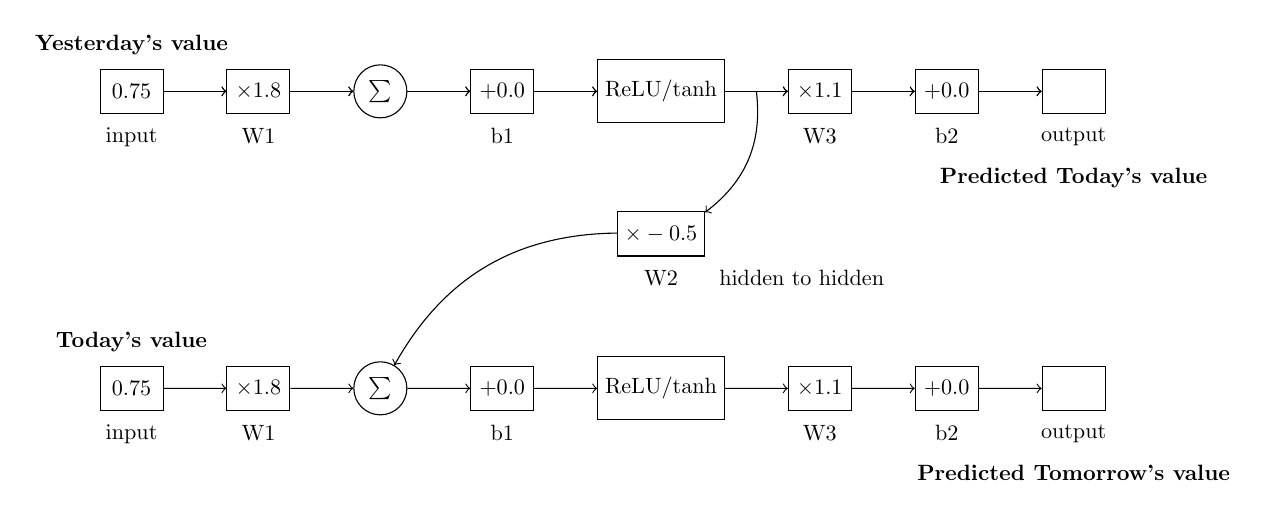
\begin{tikzpicture}[scale=0.8, transform shape, node distance=1cm, auto]
        % Input layer
        \node (input) [rectangle, draw, minimum width=1cm, minimum height=0.7cm] {$0.75$};
        \node (input_text) [below=0.1cm of input] {input};
        \node (input_text_label) [above=0.1cm of input] {\textbf{Yesterday's value}};

        % Weight W1
        \node (W1) [rectangle, draw, minimum width=1cm, minimum height=0.7cm, right=of input] {$\times 1.8$};
		\node (W1text) [below=0.1cm of W1] {W1};
		
        % Summation
        \node (sum) [circle, draw, minimum size=0.5cm, right=of W1] {$\sum$};

        % Bias b1
        \node (b1) [rectangle, draw, minimum width=1cm, minimum height=0.7cm, right=of sum] {$+0.0$};
        \node (b1text) [below=0.1cm of b1] {b1};

        % Activation function
        \node (activation) [rectangle, draw, minimum width=1.5cm, minimum height=1cm, right=of b1] {ReLU/tanh};
        

        % Weight W3
        \node (W3) [rectangle, draw, minimum width=1cm, minimum height=0.7cm, right=of activation] {$\times 1.1$};
        \node (W3text) [below=0.1cm of W3] {W3};

        % Bias b2
        \node (b2) [rectangle, draw, minimum width=1cm, minimum height=0.7cm, right=of W3] {$+0.0$};
          \node (b2text) [below=0.1cm of b2] {b2};


        % Output layer
        \node (output) [rectangle, draw, minimum width=1cm, minimum height=0.7cm, right=of b2] {};
        \node (output_text) [below=0.1cm of output] {output};
        \node (output_text_label) [below=0.1cm of output_text] {\textbf{Predicted Today's value}};

      
        
        % Second row nodes (copies with "_2" suffix)
    \node (input_2) [rectangle, draw, minimum width=1cm, minimum height=0.7cm, below=4cm of input] {$0.75$};
    \node (input_text_2) [below=0.1cm of input_2] {input};
    \node (input_text_2_label) [above=0.1cm of input_2] {\textbf{Today's value}};

    % Weight W1_2
    \node (W1_2) [rectangle, draw, minimum width=1cm, minimum height=0.7cm, right=of input_2] {$\times 1.8$};
    \node (W1text_2) [below=0.1cm of W1_2] {W1};
    
    % Summation_2
    \node (sum_2) [circle, draw, minimum size=0.5cm, right=of W1_2] {$\sum$};

    % Bias b1_2
    \node (b1_2) [rectangle, draw, minimum width=1cm, minimum height=0.7cm, right=of sum_2] {$+0.0$};
    \node (b1text_2) [below=0.1cm of b1_2] {b1};

    % Activation function_2
    \node (activation_2) [rectangle, draw, minimum width=1.5cm, minimum height=1cm, right=of b1_2] {ReLU/tanh};
    
    % Weight W3_2
    \node (W3_2) [rectangle, draw, minimum width=1cm, minimum height=0.7cm, right=of activation_2] {$\times 1.1$};
    \node (W3text_2) [below=0.1cm of W3_2] {W3};

    % Bias b2_2
    \node (b2_2) [rectangle, draw, minimum width=1cm, minimum height=0.7cm, right=of W3_2] {$+0.0$};
    \node (b2text_2) [below=0.1cm of b2_2] {b2};

    % Output layer_2
    \node (output_2) [rectangle, draw, minimum width=1cm, minimum height=0.7cm, right=of b2_2] {};
    \node (output_text_2) [below=0.1cm of output_2] {output};
    \node (output_text_2_label) [below=0.1cm of output_text_2] {\textbf{Predicted Tomorrow's value}};

    % Feedback connection (W2)_2
    \coordinate (feedback_start_2) at ([xshift=0.5cm]activation_2.east); % Point after activation
    
      % Feedback connection (W2)
        \coordinate (feedback_start) at ([xshift=0.5cm]activation.east); % Point after activation
        
        \node (W2) [rectangle, draw, minimum width=1cm, minimum height=0.7cm, below=1.4cm of activation] {$\times -0.5$};
        \node (hidden_text) [below=0.1cm of W2] {W2};
        \node (hidden_to_hidden_text) [below right=0.1cm and 0.1cm of W2] {hidden to hidden};

        % Arrows
        \draw [->] (input) -- (W1);
        \draw [->] (W1) -- (sum);
        \draw [->] (sum) -- (b1);
        \draw [->] (b1) -- (activation);
        \draw [->] (activation) -- (W3);
        \draw [->] (W3) -- (b2);
        \draw [->] (b2) -- (output);
        \draw [->] (feedback_start) to[bend left] (W2);
        \draw [->] (W2) to[bend right] (sum_2);

    % Connections for first row
    \draw[->] (input) -- (W1);
    \draw[->] (W1) -- (sum);
    \draw[->] (sum) -- (b1);
    \draw[->] (b1) -- (activation);
    \draw[->] (activation) -- (W3);
    \draw[->] (W3) -- (b2);
    \draw[->] (b2) -- (output);

    % Connections for second row
    \draw[->] (input_2) -- (W1_2);
    \draw[->] (W1_2) -- (sum_2);
    \draw[->] (sum_2) -- (b1_2);
    \draw[->] (b1_2) -- (activation_2);
    \draw[->] (activation_2) -- (W3_2);
    \draw[->] (W3_2) -- (b2_2);
    \draw[->] (b2_2) -- (output_2);


    \end{tikzpicture}
  
  
\end{frame}

\begin{frame}{}
%  \begin{center}
%   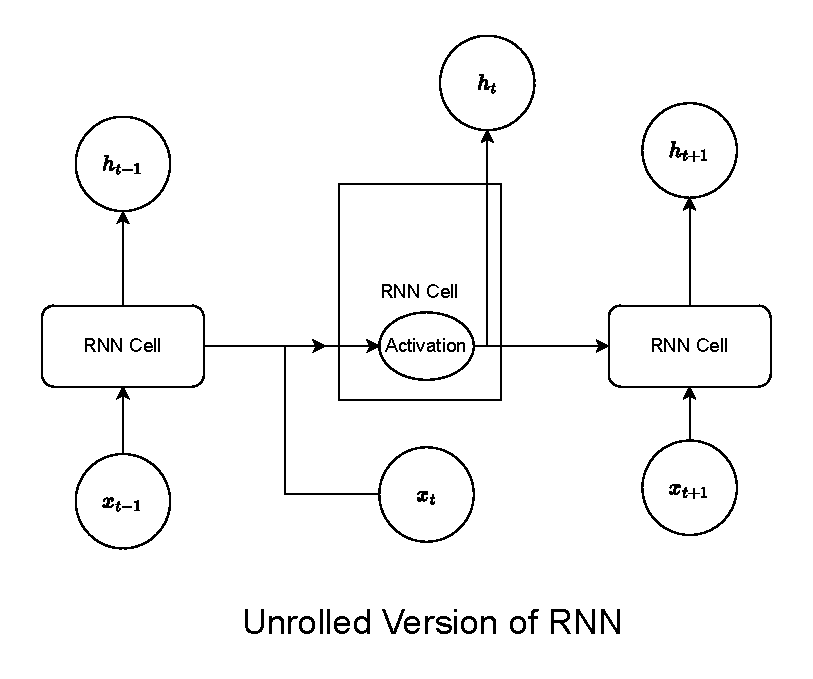
\includegraphics[width=0.6\textwidth]{figures/unrolled_RNN.pdf}
%  \end{center}
\begin{center}
   \includegraphics[width=1.0\textwidth]{figures/RNNfull.png}
  \end{center}
  
  Source: \url{https://github.com/dvgodoy/dl-visuals}


\end{frame}


\begin{frame}{Teacher Forcing}
  The idea that the predicted value is not used as input but the true value is used is called \textbf{teacher forcing}.

 \end{frame}
 
  \begin{frame}{Vanishing Gradient / Exploding Gradient Problem}
  As we see that when we unroll the network, we have multiplication of $W_2$ (recurrent weight) with itself many times.
  
  \begin{tblock}{Exploding Gradient}
     If $W_2 > 1$, then eventually, the gradient will become really large ($W_2^{50} \gg 1$).
  \end{tblock}

 \begin{tblock}{Vanishing Gradient}
     If $W_2 < 1$, then eventually, the gradient will become really small ($W_2^{50} \ll 1$).
  \end{tblock}



\end{frame}


\begin{frame}{Vanishing Gradient / Exploding Gradient Problem}
Consider an RNN with ReLU activation:
  \begin{multiequation}
    h_t &= \max(0, W_1 x_t + W_2 h_{t-1} + b_1) \\
    y_t &= W_3 h_t + b_2
  \end{multiequation}
  The backpropagation through time (BPTT) is used for training sequence data.

  The gradient of the loss ($L$) with respect to $W_2$ is:
  $$
  \frac{\partial L}{\partial W_2} = \sum_{k=1}^{t} \frac{\partial L}{\partial y_k} \cdot \frac{\partial y_k}{\partial h_k} \cdot \frac{\partial h_k}{\partial W_2}
  $$
  where $k$ is the index for time.
  
\end{frame}

\begin{frame}{Vanishing Gradient / Exploding Gradient Problem}

  $$
  \frac{\partial h_k}{\partial W_2} = \frac{\partial h_k}{\partial h_{k-1}}\cdot \frac{\partial h_{k-1}}{\partial W_2} = W_2\cdot  \frac{\partial h_{k-1}}{\partial W_2}  = W_2 \cdot \left( W_2 \cdot \frac{\partial h_{k-2}}{\partial W_2} \right) = W_2^2 \cdot \frac{\partial h_{k-2}}{\partial W_2}
  $$
  Continuing this pattern, we get:
  $$
  \frac{\partial h_k}{\partial W_2} = W_2^{k-1} \cdot \frac{\partial h_1}{\partial W_2}
  $$
  This shows that the gradient $\frac{\partial h_k}{\partial W_2}$ is proportional to $W_2$ and the previous gradients.

  \bigskip
  As you see, if $|W_2| > 1$, then the gradient grows exponentially (exploding gradient).

  \bigskip
  If $|W_2| < 1$, then the gradient vanishes.
\end{frame}

\begin{frame}{Long Short-Term Memory(LSTM)}
  In LSTM, we modify connections, so that there are two separate paths for long-term dependencies and short-term dependencies.

\begin{columns}
\column{0.3\linewidth}
\begin{itemize}
\item LSTM specifically uses the tanh and sigmoid activation functions:

\end{itemize}
  $$
  \tanh(x) = \frac{e^x - e^{-x}}{e^x + e^{-x}}
  $$
  $$
  \text{sigmoid}(x) = \frac{1}{1 + e^{-x}}
  $$
  \column{0.7\linewidth}
    \begin{center}
   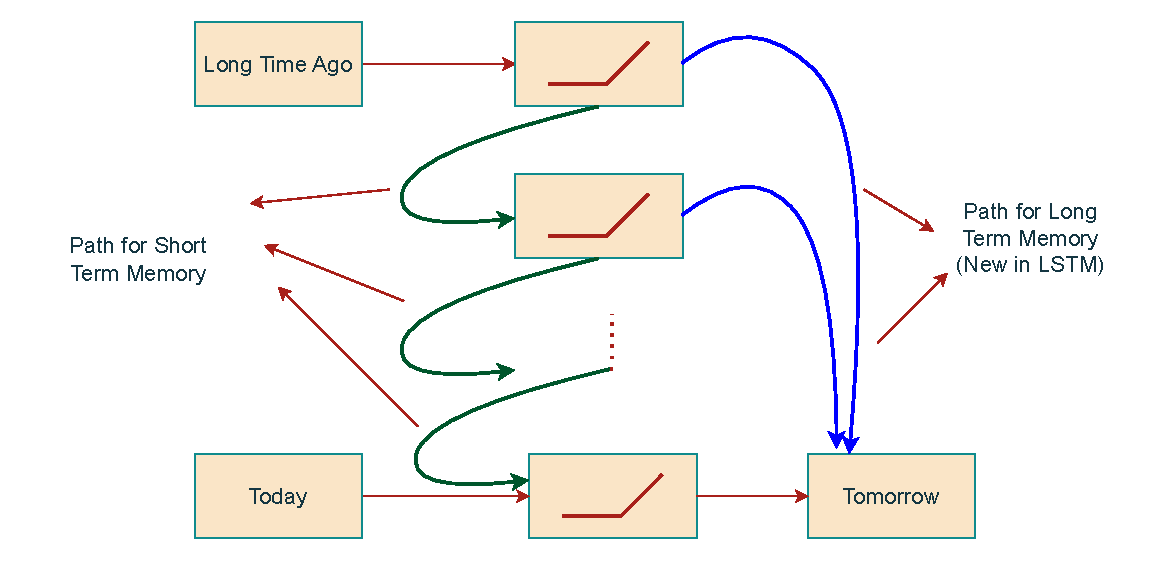
\includegraphics[width=1.0\textwidth]{figures/LSTM.pdf}
  \end{center}
\end{columns}


\end{frame}

\begin{frame}{LSTM}
    \begin{center}
   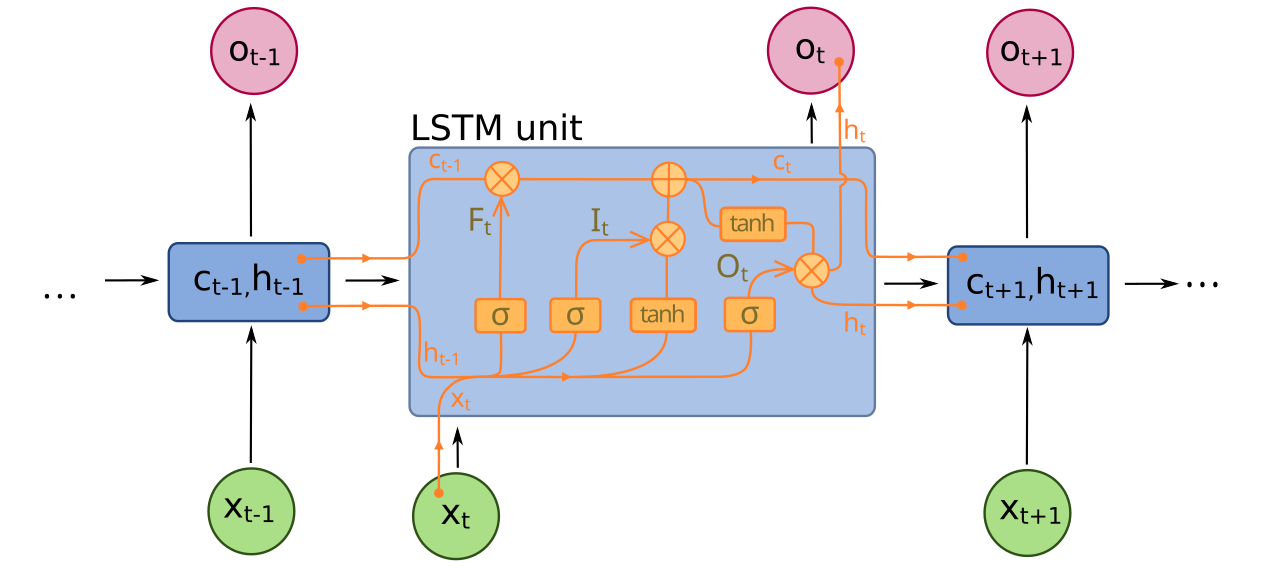
\includegraphics[width=0.8\textwidth]{figures/LSTM.png}
  \end{center}
  
    Source: \url{https://github.com/dvgodoy/dl-visuals}


\end{frame}

\begin{frame}{What's special in LSTM}
\begin{tblock}{Central Idea}
LSTM Introduces cell state and gating mechanisms to preserve long-term information. A memory cell (interchangeably block) which can maintain its state over time, consisting of an explicit memory (aka the cell state vector) and gating units which regulate the information flow into and out of the memory.
\end{tblock}
 
 There are 3 kinds of gating mechanism:
  \begin{itemize}
    \item \textbf{Forget Gate}: Decides what information to discard
    \item \textbf{Input Gate}: Decides what new information to store
    \item \textbf{Output Gate}: Decides what to output
  \end{itemize}


\end{frame}

\begin{frame}{LSTM Memory Cell}
 \begin{center}
   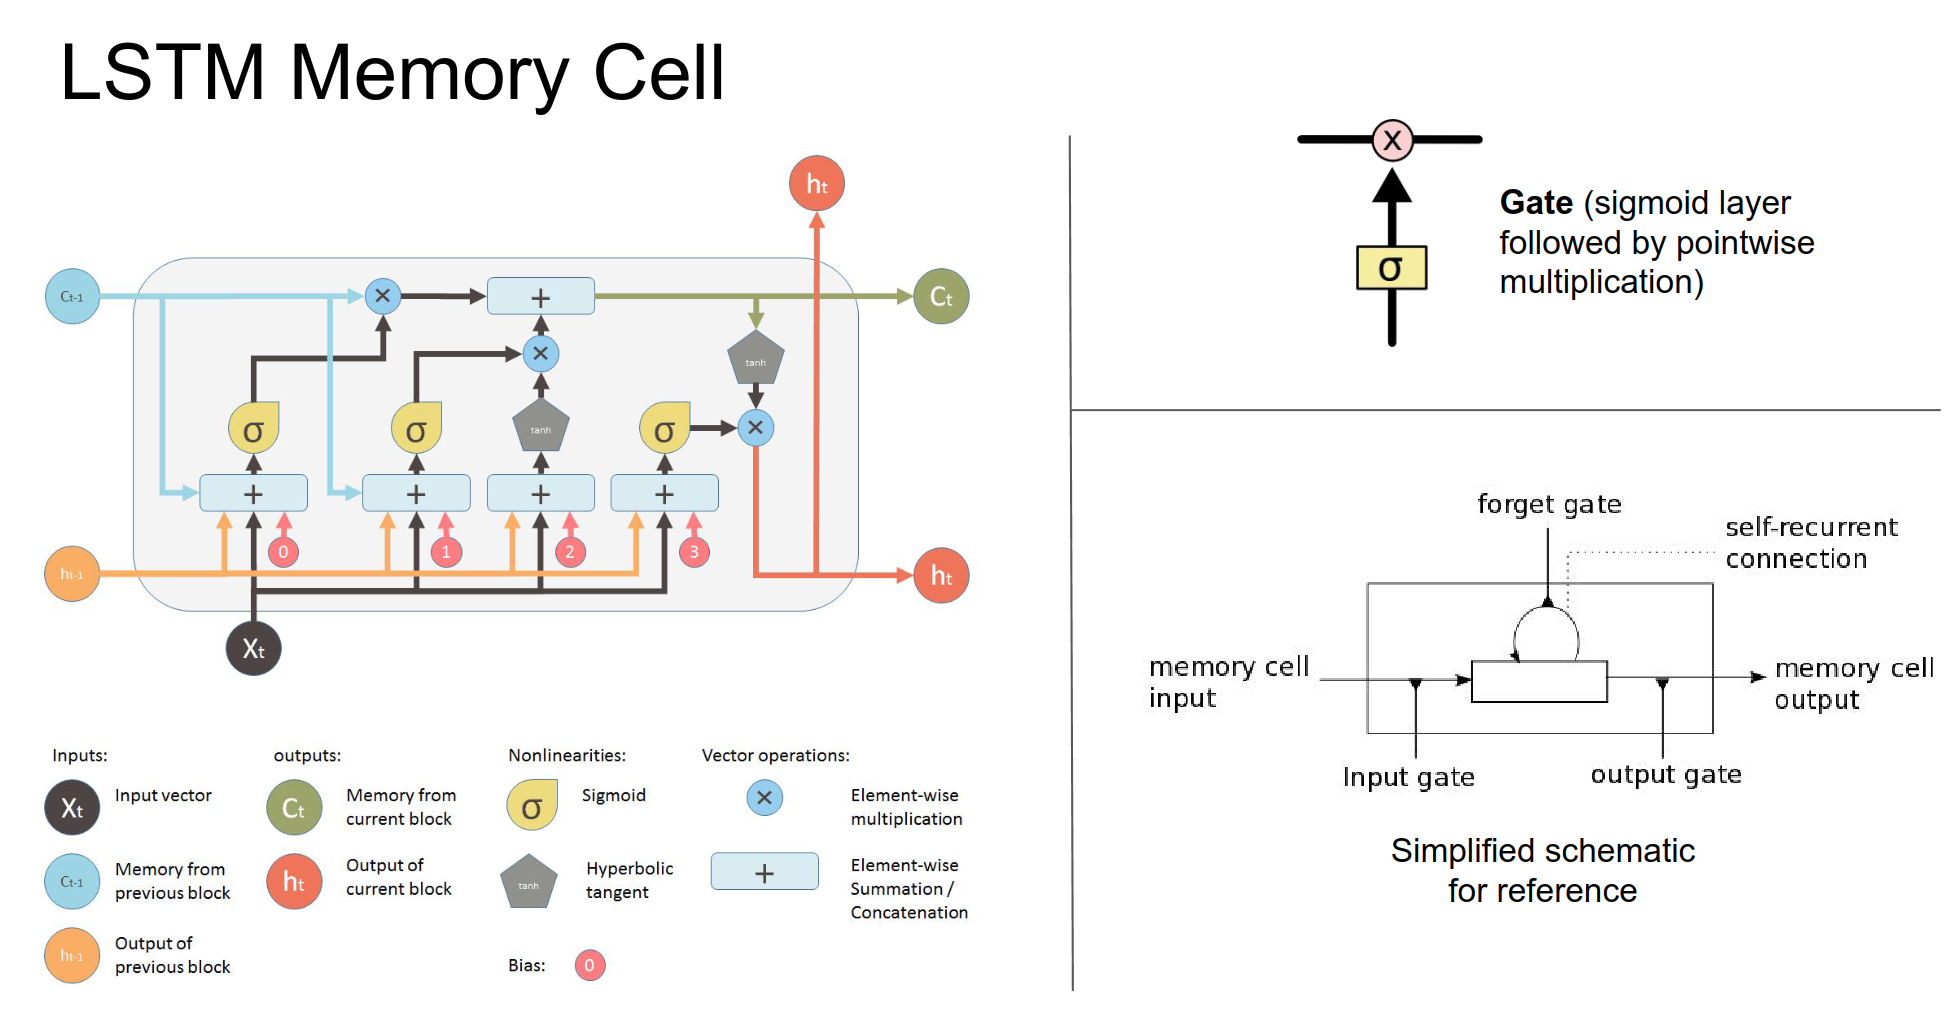
\includegraphics[width=0.7\textwidth]{figures/LSTMMemoryCell.png}
  \end{center}
  \tiny
  Source: \url{https://pages.cs.wisc.edu/~shavlik/cs638/lectureNotes/Long\%20Short-Term\%20Memory\%20Networks.pdf}
  
\end{frame}

\begin{frame}{Forget Gate}
\begin{center}
   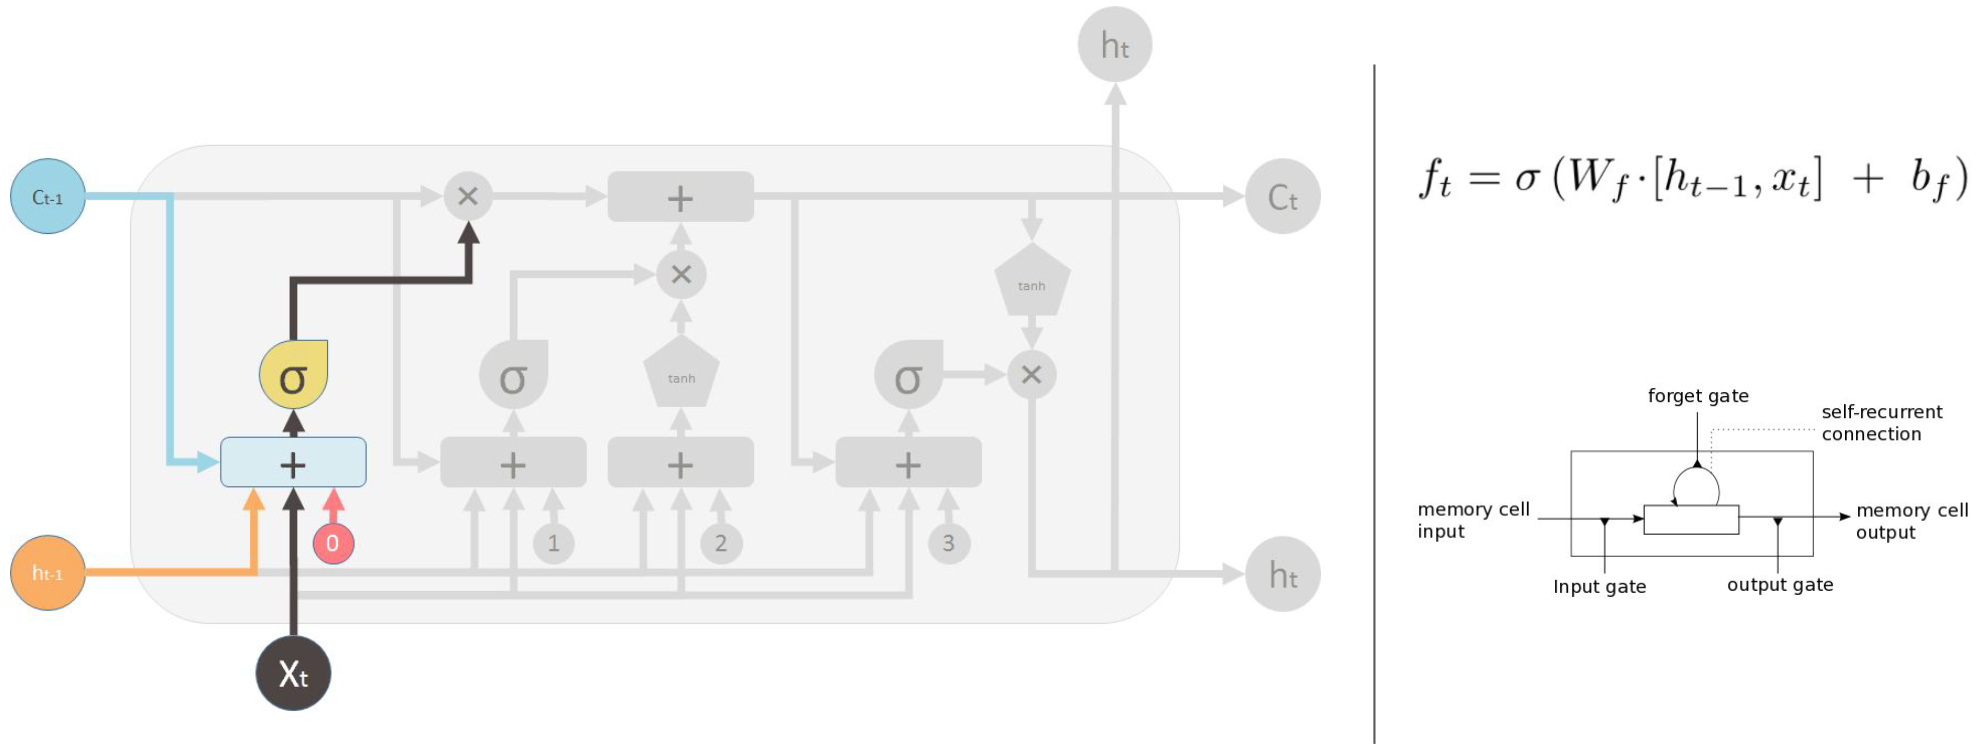
\includegraphics[width=0.8\textwidth]{figures/forgetgate.png}
  \end{center}
  \tiny
  Source: \url{https://pages.cs.wisc.edu/~shavlik/cs638/lectureNotes/Long\%20Short-Term\%20Memory\%20Networks.pdf}
\end{frame}


\begin{frame}{Input Gate}
\begin{center}
   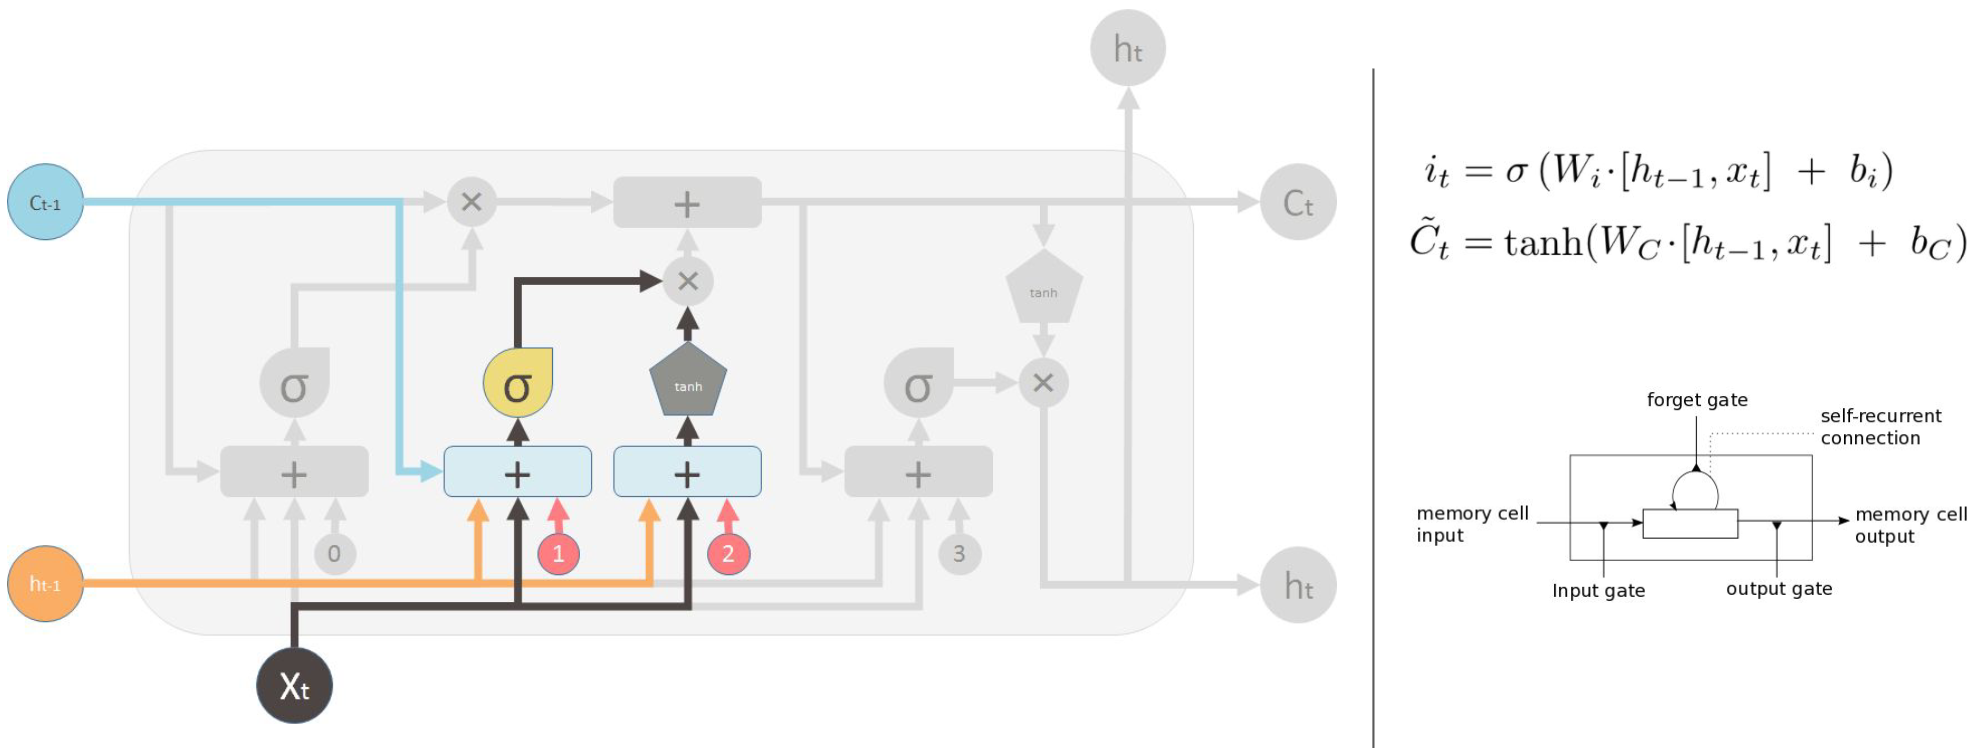
\includegraphics[width=0.8\textwidth]{figures/inputgate.png}
  \end{center}
  \tiny
  Source: \url{https://pages.cs.wisc.edu/~shavlik/cs638/lectureNotes/Long\%20Short-Term\%20Memory\%20Networks.pdf}

\end{frame}


\begin{frame}{Memory Update}
The cell state vector aggregates the two components (old memory via the
forget gate and new memory via the input gate)
\begin{center}
   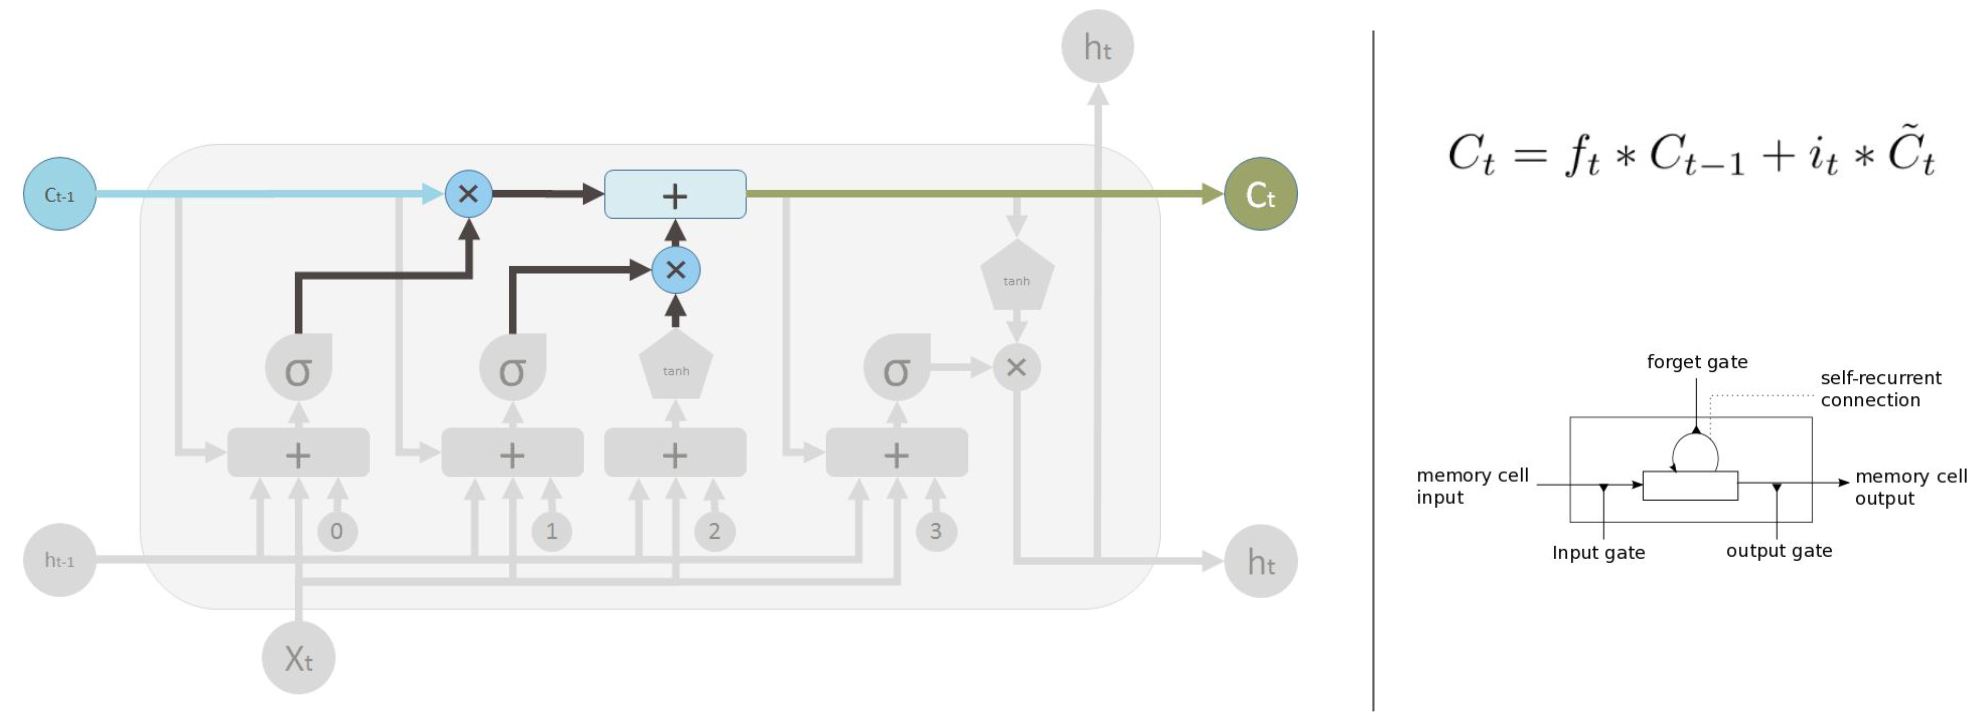
\includegraphics[width=0.8\textwidth]{figures/memoryupdate.png}
  \end{center}
  \tiny
  Source: \url{https://pages.cs.wisc.edu/~shavlik/cs638/lectureNotes/Long\%20Short-Term\%20Memory\%20Networks.pdf}

\end{frame}

\begin{frame}{Output Gate}
\begin{center}
   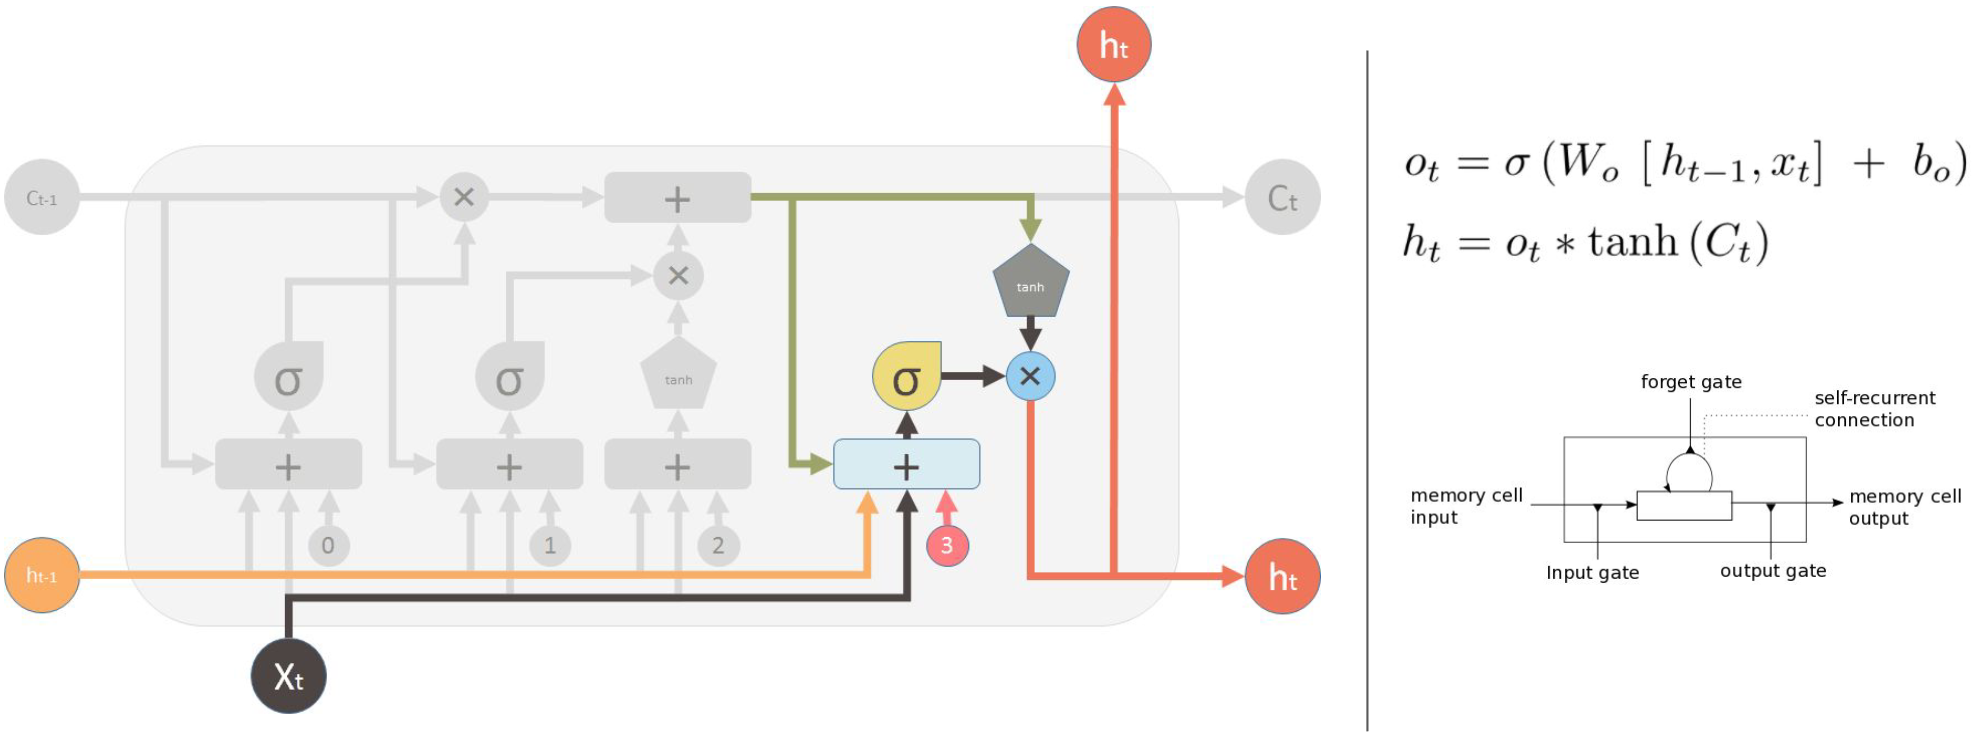
\includegraphics[width=0.8\textwidth]{figures/outputgate.png}
  \end{center}
  \tiny
  Source: \url{https://pages.cs.wisc.edu/~shavlik/cs638/lectureNotes/Long\%20Short-Term\%20Memory\%20Networks.pdf}

\end{frame}


\begin{frame}{References}

\begin{enumerate}
\item \url{https://web.stanford.edu/~jurafsky/slp3/3.pdf}
\end{enumerate}

\end{frame}

\end{document}